\documentclass{article}

% Packages
\usepackage{amsmath}
\usepackage{array}
\usepackage{enumitem}
\usepackage{float}
\usepackage[T1]{fontenc}
\usepackage{geometry}
\usepackage{graphicx}
\usepackage[colorlinks=true,linkcolor=blue,urlcolor=blue,citecolor=blue]{hyperref}     
\usepackage[utf8]{inputenc}
\usepackage{listings}
\usepackage{tabularx}
\usepackage{tcolorbox}
\usepackage{tikz}
\usepackage{xcolor}
\usepackage[table]{xcolor}
\usepackage{verbatim}

% Define levels of depth
\setcounter{secnumdepth}{5} % Numbering up to subsection 5
\setcounter{tocdepth}{3} % Include up to subsection 5 in the table of contents

% Define colors
\definecolor{grayheavy}{gray}{0.7}
\definecolor{graylight}{gray}{0.8}
\definecolor{graysuperlight}{gray}{0.9}

\usetikzlibrary{shapes.geometric}
\usetikzlibrary{positioning}  

% Page layout
\geometry{margin=1in}

\tikzstyle{startstop} = [rectangle, rounded corners, minimum width=3cm, minimum height=1cm,text centered, draw=black, fill=red!30]
\tikzstyle{process} = [rectangle, minimum width=3cm, minimum height=1cm, text centered, draw=black, fill=blue!30]
\tikzstyle{condition} = [diamond, minimum width=3cm, minimum height=1cm, text centered, draw=black, fill=white!100]
\tikzstyle{file} = [rectangle, minimum width=3cm, minimum height=1cm, text centered, draw=black, fill=gray!30]
\tikzstyle{arrow} = [thick,->,>=stealth]  
\tikzstyle{line} = [thick,-,>=stealth]  

% Functions
\tcbset{
    attentionbox/.style={
        colback=red!5, % Background color
        colframe=red!75!black, % Border color
        coltitle=black, % Title color
        boxrule=0.8mm, % Thickness of the border
        left=2mm, % Left padding
        before skip=5mm, % Space before the box
        after skip=5mm, % Space after the box
        sharp corners, % Sharp corners for the box
        fonttitle=\bfseries, % Bold title font
        attach boxed title to top left={yshift=-2mm,xshift=2mm}, % Title position
        boxed title style={
            size=small,
            colback=red!50,
            colframe=red!75!black,
            sharp corners,
        },
    }
}

% % Code formatting
\lstset{
    language=Python,
    basicstyle=\ttfamily\fontsize{9}{10}\selectfont,
    breaklines=true,
    frame=single,
    keywordstyle=\color{blue},
    commentstyle=\color{green!70!black},
    stringstyle=\color{red},
    showstringspaces=false,
    numbers=left,
    numberstyle=\tiny\color{gray},
    stepnumber=1,
    numbersep=10pt,
    xleftmargin=5mm,
}

\lstdefinelanguage{json}{
    basicstyle=\ttfamily,
    numbers=left,
    numberstyle=\tiny,
    stepnumber=1,
    numbersep=5pt,
    showstringspaces=false,
    breaklines=true,
    frame=single,
    backgroundcolor=\color{white},
    literate=
     *{0}{{{\color{blue}0}}}{1}
      {1}{{{\color{blue}1}}}{1}
      {2}{{{\color{blue}2}}}{1}
      {3}{{{\color{blue}3}}}{1}
      {4}{{{\color{blue}4}}}{1}
      {5}{{{\color{blue}5}}}{1}
      {6}{{{\color{blue}6}}}{1}
      {7}{{{\color{blue}7}}}{1}
      {8}{{{\color{blue}8}}}{1}
      {9}{{{\color{blue}9}}}{1}
      {:}{{{\color{red}{:}}}}{1}
      {,}{{{\color{red}{,}}}}{1}
      {\{}{{{\color{yellow}{\{}}}}{1}
      {\}}{{{\color{yellow}{\}}}}}{1}
      {[}{{{\color{black}{[}}}}{1}
      {]}{{{\color{black}{]}}}}{1},
}

\newcommand{\mypart}[1]{\setcounter{chapter}{0} \part{#1}}
\renewcommand{\theHsection}{\thepart.section.\thesection}

\title{Testing the HDF5\_BLS package for creating BrimX files}
\author{Pierre Bouvet}
\date{2025}

\begin{document}

\maketitle

\tableofcontents

\section{Installation of the HDF5\_BLS package}

The HDF5\_BLS package is a Python package for creating BrimX files. It is compatible with Python 3.10 and above. 

We recommend setting up a virtual environment to install the package. This can be done using the following command:

\begin{tcolorbox}[colback=blue!5, colframe=blue!40!black, boxrule=0.5mm, sharp corners, left=2mm, right=2mm, top=1mm, bottom=1mm]
- On Mac terminal
\begin{lstlisting}
python -m venv HDF5_BLS_venv
source HDF5_BLS_venv/bin/activate 
\end{lstlisting}
\end{tcolorbox}

\begin{tcolorbox}[colback=yellow!5, colframe=yellow!40!black, boxrule=0.5mm, sharp corners, left=2mm, right=2mm, top=1mm, bottom=1mm]
- On Windows terminal
\begin{lstlisting}
python -m venv HDF5_BLS_venv
HDF5_BLS_venv\Scripts\activate
\end{lstlisting}
\end{tcolorbox}

On both OS, the package can be installed using pip:
\begin{lstlisting}
pip install HDF5_BLS
\end{lstlisting}


\section{An example}

Here we propose to create a synthetic Brillouin dataset that we'll store in a BrimX file. We will store 3 different types of synthetic data:
\begin{itemize}
    \item A single spectrum 
    \item A synthetic time evolution
    \item A spatial mapping in 2D
    \item A z-stack of a sphere
\end{itemize}

\subsection{Creating the data}

We define a DHO function to create the Brillouin spectra.

\begin{lstlisting}
def DHO(nu, nu0, gamma, a, b):
    return b + a * (gamma*nu0)**2/((nu**2-nu0**2)**2+(gamma*nu)**2)
\end{lstlisting}

We define a frequency axis to create the spectra.

\begin{lstlisting}
nu = np.linspace(-15, 15, 1024)
\end{lstlisting}

We define the values of shift and linewidth for the different datasets to create:
\begin{itemize}
    \item For the single spectrum, we set shift to 5 GHz and linewidth to 1 GHz, with an amplitude of 1 and no offset.
\begin{lstlisting}
shift_0D = 5
linewidth_0D = 1
PSD_0D = DHO(nu, shift_0D, linewidth_0D, 1, 0)
\end{lstlisting}
    \item For the synthetic time evolution spectrum, we consider a shift rising quadratically from 5 to 6 GHz over time, a linewidth raising from 1 to 2 GHz linearly, and an amplitude of 1 with no offset.
\begin{lstlisting}
time_1D = np.linspace(0, 10, 100)
shift_1D = 5 + time**2/100
linewidth_1D = np.linspace(1, 2, 100)
for s, l in zip(shift_1D, linewidth_1D):
    PSD_1D = DHO(nu, s, l, 1, 0)
\end{lstlisting}
    \item For the synthetic spatial mapping, we consider a diagonal shift gradient from 5 to 6 GHz over time, and a diagonal linewidth gradient from 1 to 2 GHz, and an amplitude of 1 with no offset.
\begin{lstlisting}
gradient_x = np.linspace(0, 1, 50)
gradient_y = np.linspace(0, 1, 50)
temp = (np.outer(gradient_y, gradient_x) + np.outer(gradient_y, gradient_x))/2
shift_2D = temp + 5
linewidth_2D = temp + 1 
PSD_2D = np.zeros((50, 50, 1024))
for i in range(50):
    for j in range(50):
        PSD_2D[i, j] = DHO(nu, shift_2D[i, j], linewidth_2D[i, j], 1, 0) 
\end{lstlisting}
    \item For the synthetic z-stack mapping, we consider a sphere with a shift of 6GHz and linewidth 2GHz in a solution of shift 5GHz and linewidth 1GHz, with an amplitude for all spectra of 1 and an offset of 0. The z-stack is made of 50 slices 
\begin{lstlisting}
x = np.linspace(-1, 1, 50)
y = np.linspace(-1, 1, 50)
z = np.linspace(-1, 1, 50)
shift_3D = np.zeros((50, 50, 50))
linewidth_3D = np.zeros((50, 50, 50))
PSD_3D = np.zeros((50, 50, 50, 1024))
for i in range(50):
    for j in range(50):
        for k in range(50):
            if (x[i]**2 + y[j]**2 + z[k]**2) > 1:
                shift_3D[i, j, k] = 5 
                linewidth_3D[i, j, k] = 1 
            else:
                shift_3D[i, j, k] = 6 
                linewidth_3D[i, j, k] = 2 
            PSD_3D[i, j, k] = DHO(nu, shift_3D[i, j, k], linewidth_3D[i, j, k], 1, 0)
\end{lstlisting}
\end{itemize}

We have provided in the joined Python script, options to visualize the created datasets.

\subsection{Adding the data to a BrimX file}

Here we're going to structure our file to store the four different datasets we've created. Each dataset will be stored in a separate group, and the group will be named with example names.

First we create the BrimX file at a given path, and define an object "wrp" to interact with it.
\begin{lstlisting}
wrp = wrapper.Wrapper('path/to/file.h5')
\end{lstlisting}

For this example, we will structure the file as follows:
\begin{verbatim}
file.h5
|- Brillouin
|  |- A single spectrum 
|  |- A time series
|  |- A mapping
|  |- A z-stack
\end{verbatim}

In each of these groups, we will store the corresponding Power spectral density datasets, frequency array and shift and linewidth arrays. To do so, we will use the following code:
\begin{lstlisting}
# Adding the 0D datasets
wrp.add_frequency(data=nu, parent_group="Brillouin/A single spectrum", name = "Frequency")
wrp.add_PSD(data=PSD_0D, parent_group="Brillouin/A single spectrum", name = "PSD")
wrp.add_treated_data(parent_group="Brillouin/A single spectrum", name_group = "Treated Data", shift = shift_0D, linewidth = linewidth_0D)

# Adding the 1D datasets
wrp.add_frequency(data=nu, parent_group="Brillouin/A time series", name = "Frequency")
wrp.add_PSD(data=PSD_1D, parent_group="Brillouin/A time series", name = "PSD")
wrp.add_treated_data(parent_group="Brillouin/A time series", name_group = "Treated Data", shift = shift_1D, linewidth = linewidth_1D)

# Adding the 2D datasets
wrp.add_frequency(data=nu, parent_group="Brillouin/A mapping", name = "Frequency")
wrp.add_PSD(data=PSD_2D, parent_group="Brillouin/A mapping", name = "PSD")
wrp.add_treated_data(parent_group="Brillouin/A mapping", name_group = "Treated Data", shift = shift_2D, linewidth = linewidth_2D)

# Adding the 3D datasets
wrp.add_frequency(data=nu, parent_group="Brillouin/A z-stack", name = "Frequency")
wrp.add_PSD(data=PSD_3D, parent_group="Brillouin/A z-stack", name = "PSD")
wrp.add_treated_data(parent_group="Brillouin/A z-stack", name_group = "Treated Data", shift = shift_3D, linewidth = linewidth_3D)
\end{lstlisting}

You are now the proud owner of a BrimX file containing synthetic Brillouin datasets!

\subsection{Adding metadata to the BrimX file}

To add metadata to the BrimX file, we will choose the easy way for this example, and just edit the standard spreadsheet given with the package and downloadable at this link: \url{https://github.com/bio-brillouin/HDF5_BLS/blob/main/spreadsheets/attributes_v1.0.xlsx}.

A list of established parameters is given, their name, units and definition is written in the different columns. For this example, we are filling the datasheet as presented on figure \ref{fig:excel_attributes}.
\begin{figure}[H]
    \centering
    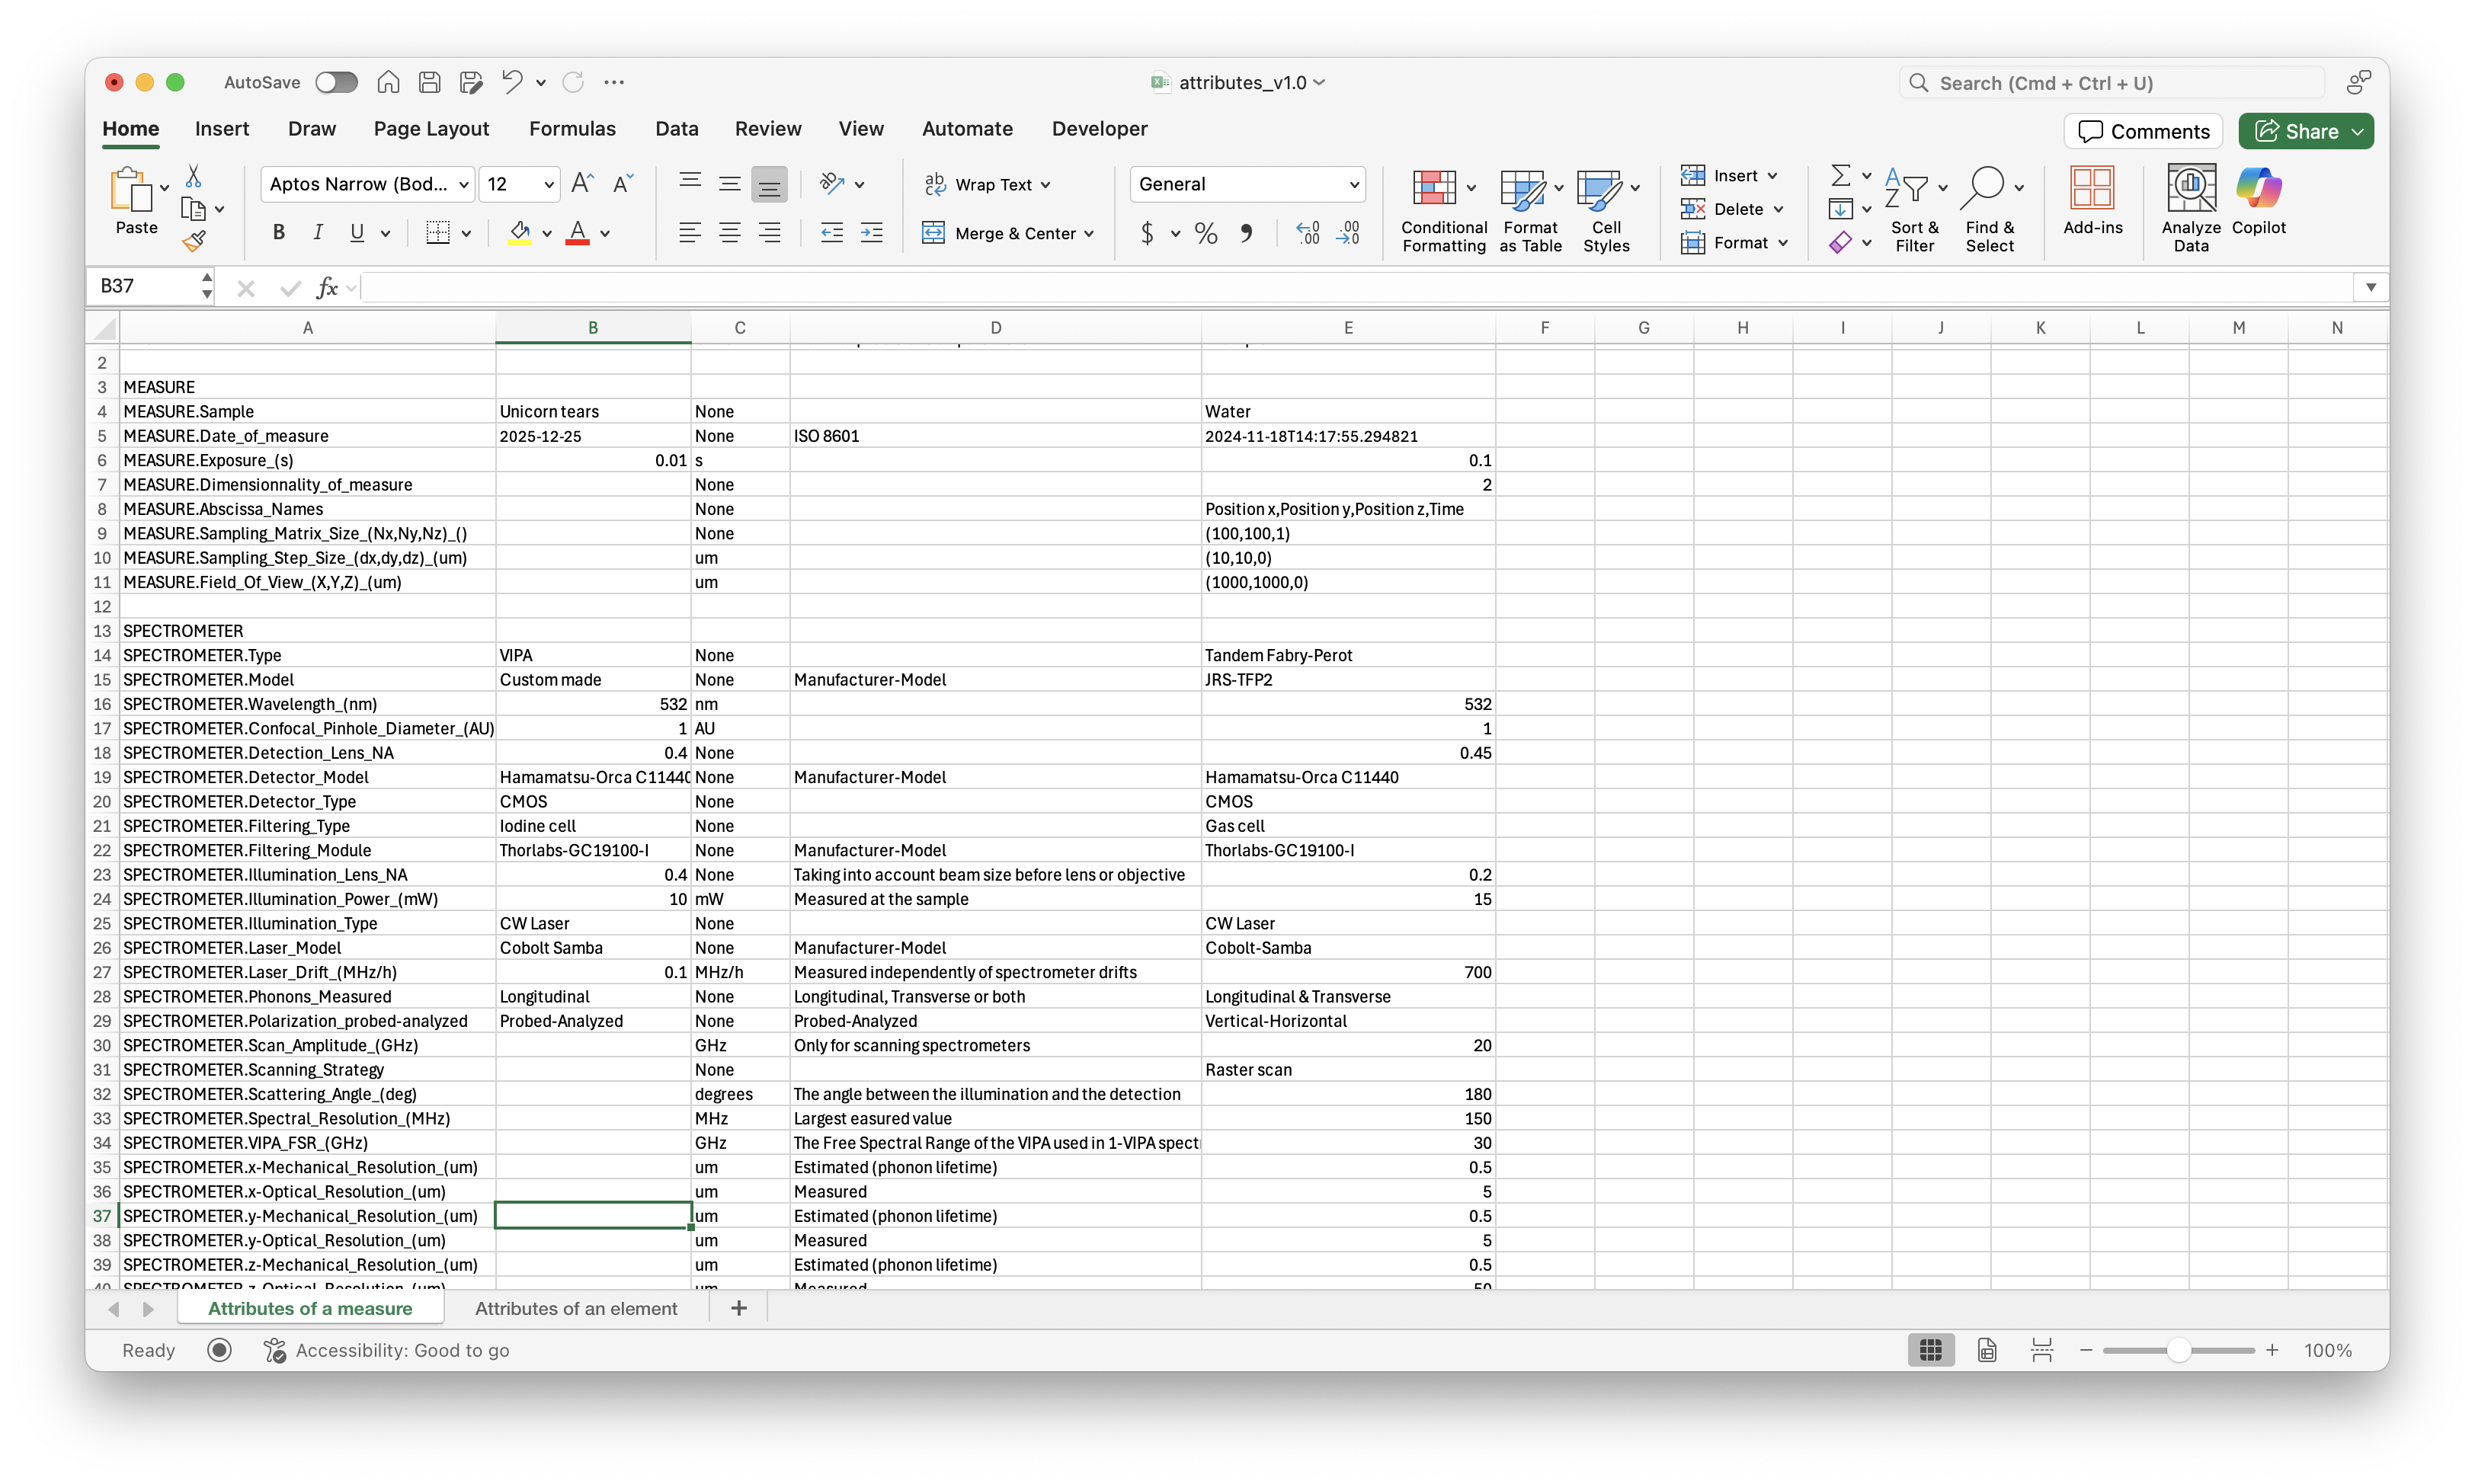
\includegraphics[width=\textwidth]{img/Excel_attributes.png}
    \caption{Example of the filled datasheet used to add metadata to the BrimX file}
    \label{fig:excel_attributes}
\end{figure}

You can of course play with this file, add your own parameters, change the values for the ones given, add values for the ones not given, etc. We recommend however not changing the name of the parameters so that all the community calls the same parameters the same way.

You can then save the file at your prefered location, and apply it to the BrimX file you just created. To do so, you can use the following code:

\begin{lstlisting}
wrp.import_properties_data(filepath='local_use/example_attributes.xlsx')
\end{lstlisting}

This line of code applies the metadata to the whole BrimX file. You can also apply metadata to a specific group by adding the argument "parent\_group" to the function:

\begin{lstlisting}
wrp.import_properties_data(filepath='local_use/example_attributes.xlsx', path = "Brillouin/A z-stack")
\end{lstlisting}


\section{Template for integrating BrimX files to your workflow}

You can now try integrating the use of BrimX files in your workflow. Note that the example we showed above is limited to 4 kinds of datasets (frequency, PSD, shift and linewidth). The format can handle a total of 13 different kinds of datasets that are defined in the documentation of the package: \url{https://github.com/bio-brillouin/HDF5_BLS/blob/main/guides/Tutorial/Tutorial.pdf}.

Here is a base template to get you started:

\begin{lstlisting}
import HDF5_BLS as bls

# Create a BrimX file
wrp = bls.Wrapper(filepath = "path/to/file.h5")

###############################################################################
# Existing code to extract data from a file
###############################################################################
# Storing the data in the HDF5 file (for this example we use a random array)
data = np.random.random((50, 50, 512))
wrp.add_raw_data(data = data, parent_group = "Brillouin", name = "Raw data")

###############################################################################
# Existing code to convert the data to a PSD
###############################################################################
# Storing the Power Spectral Density in the HDF5 file together with the associated frequency array (for this example we use random arrays)
PSD = np.random.random((50, 50, 512))
frequency = np.arange(512)
wrp.add_PSD(data = PSD, parent_group = "Brillouin", name = "Power Spectral Density")
wrp.add_frequency(data = frequency, parent_group = "Brillouin", name = "Frequency")

###############################################################################
# Existing code to fit the PSD to extract shift and linewidth arrays
###############################################################################
# Storing the Power Spectral Density in the HDF5 file together with the associated frequency array (for this example we use random arrays)
shift = np.random.random((50, 50))
linewidth = np.random.random((50, 50))
wrp.add_treated_data(parent_group = "Brillouin", name_group = "Treat_0", shift = shift, linewidth = linewidth)
\end{lstlisting}

\section{Extracting data from the BrimX file}

You can now interact directly with the BrimX file as any other file storing data. To extract a dataset located at a known path in the file, you can use the following line of code:
\begin{lstlisting}
dataset = wrp["path/to/dataset/in/the/file"][:]
\end{lstlisting}

For example, using the example BrimX file we created in this tutorial, you can extract the PSD of the first spectrum using the following code:
\begin{lstlisting}
psd = wrp["Brillouin/A single spectrum/PSD"][:]
\end{lstlisting}

The paths can be obtained by visualizing the file as explained in the next section.

\section{Visualizing the BrimX file}

\subsection{Online}

You can visualize the BrimX file online using the myhdf5 web application: \url{https://myhdf5.hdfgroup.org}. This application runs locally in your web browser so you can use it safely even to observe sensitive data.

When you open the application, you can upload your BrimX file and explore its contents either by clicking the "Select HDF5 File" button or by dragging and dropping your file in the window (figure \ref{fig:my_hdf5_welcome}). 

\begin{figure}[H]
    \centering
    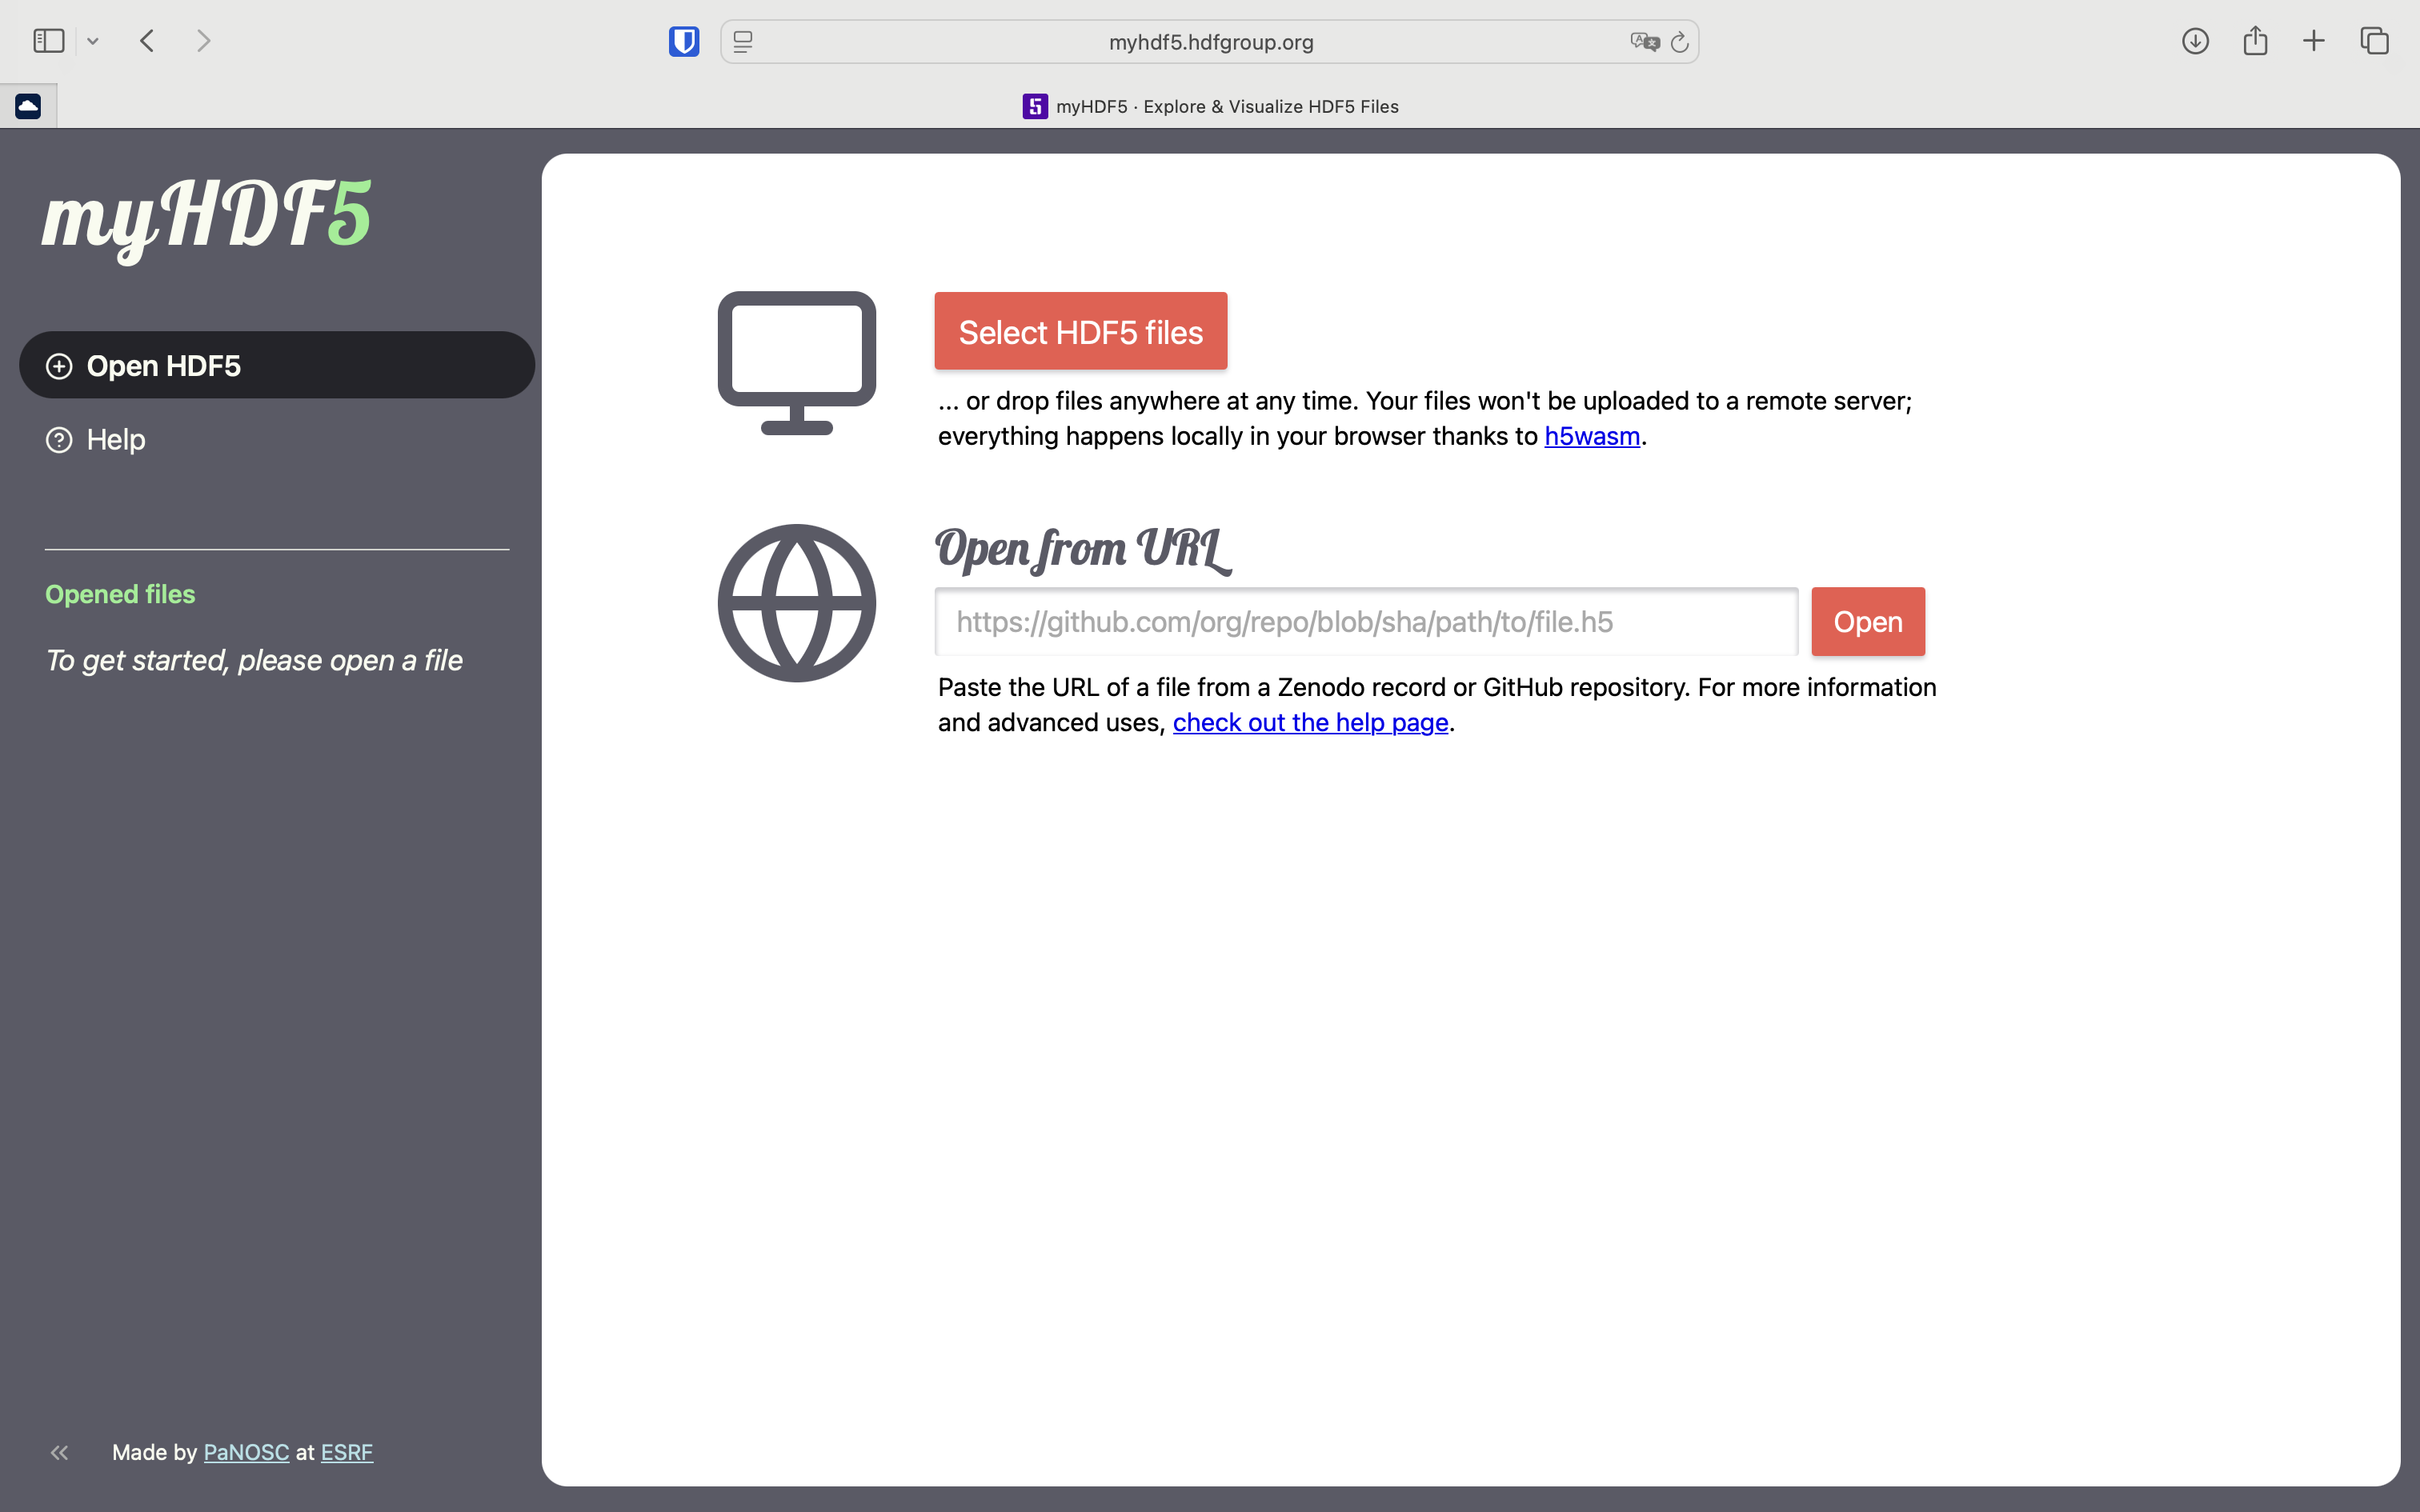
\includegraphics[width=0.8\textwidth]{img/MyHDF5_welcome_window.png}
    \caption{The welcome window of the myhdf5 application}
    \label{fig:my_hdf5_welcome}
\end{figure}

Once your file is loaded, you can explore its contents on the left panel (figure \ref{fig:my_hdf5_structure}).

\begin{figure}[H]
    \centering
    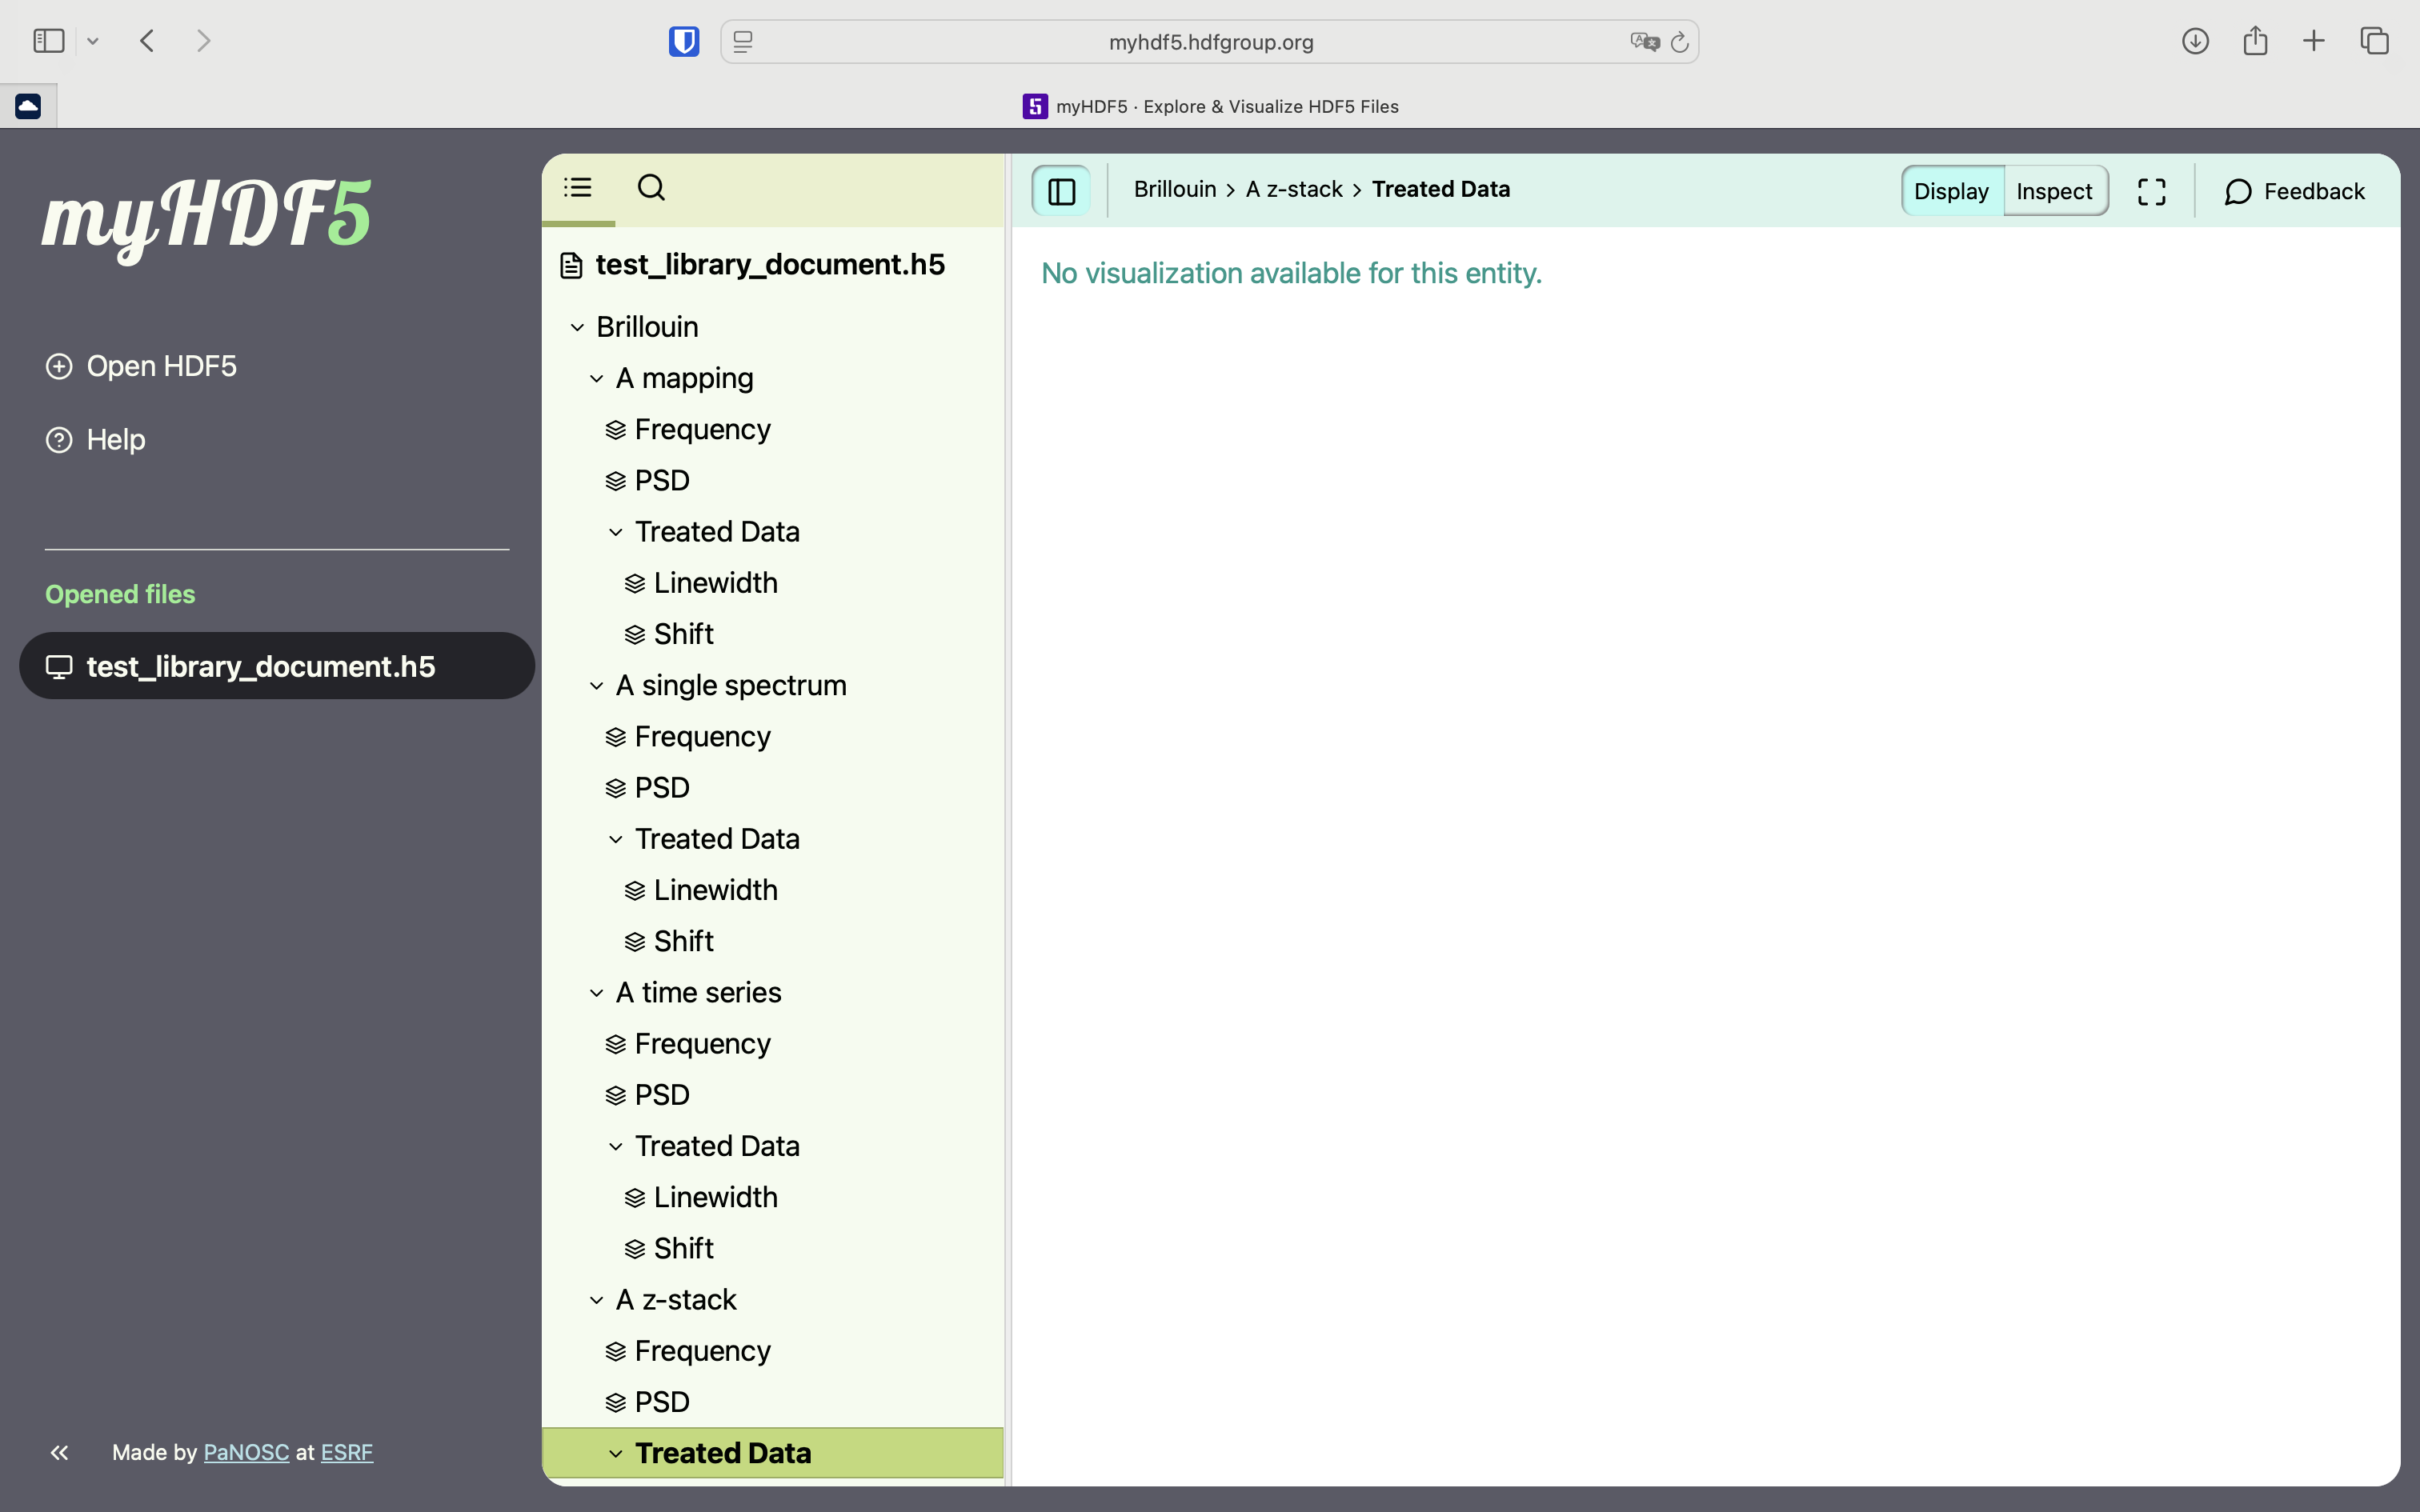
\includegraphics[width=0.8\textwidth]{img/MyHDF5_Developped structure.png}
    \caption{The developed structure view of your HDF5 file in the myhdf5 application}
    \label{fig:my_hdf5_structure}
\end{figure}

From there you can explore the file, visualize attributes (figure \ref{fig:my_hdf5_attributes}) and datasets of any dimension (figure \ref{fig:my_hdf5_datasets}).

\begin{figure}[H]
    \centering
    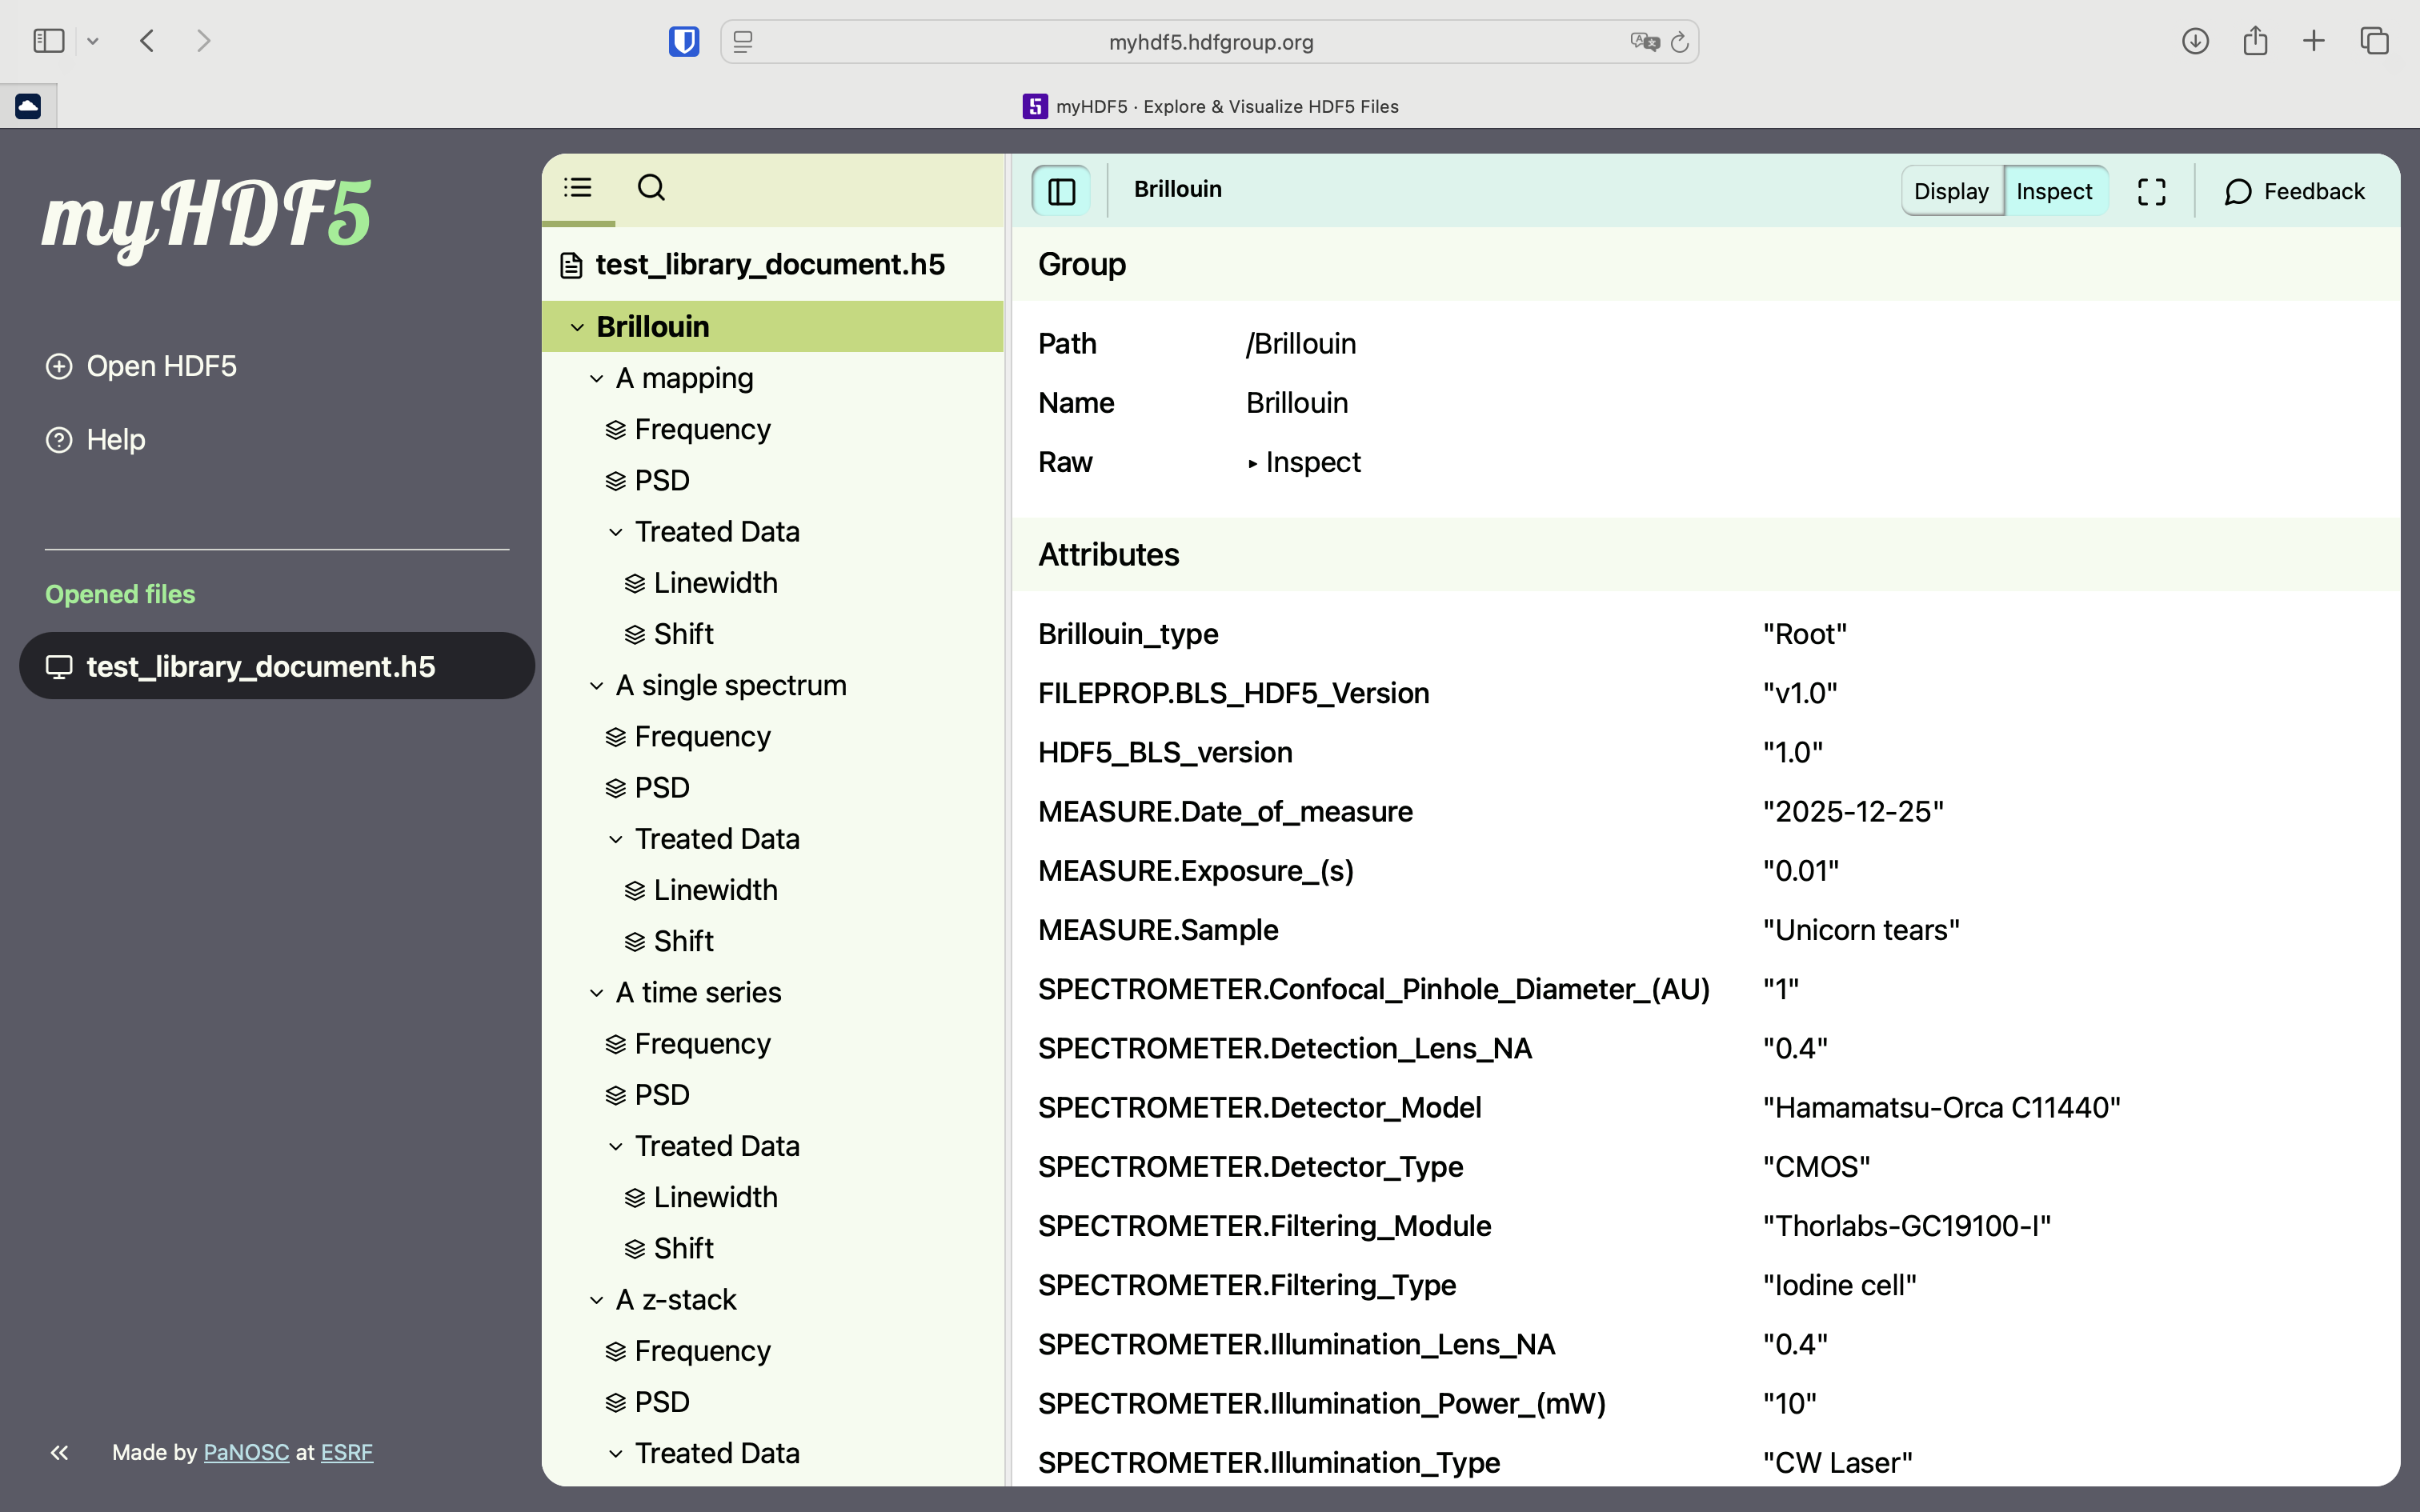
\includegraphics[width=0.8\textwidth]{img/My_HDF5_attributes.png}
    \caption{Visualizing the attributes stored in the "Brillouin" group} 
    \label{fig:my_hdf5_attributes}
\end{figure}

\begin{figure}[H]
    \centering
    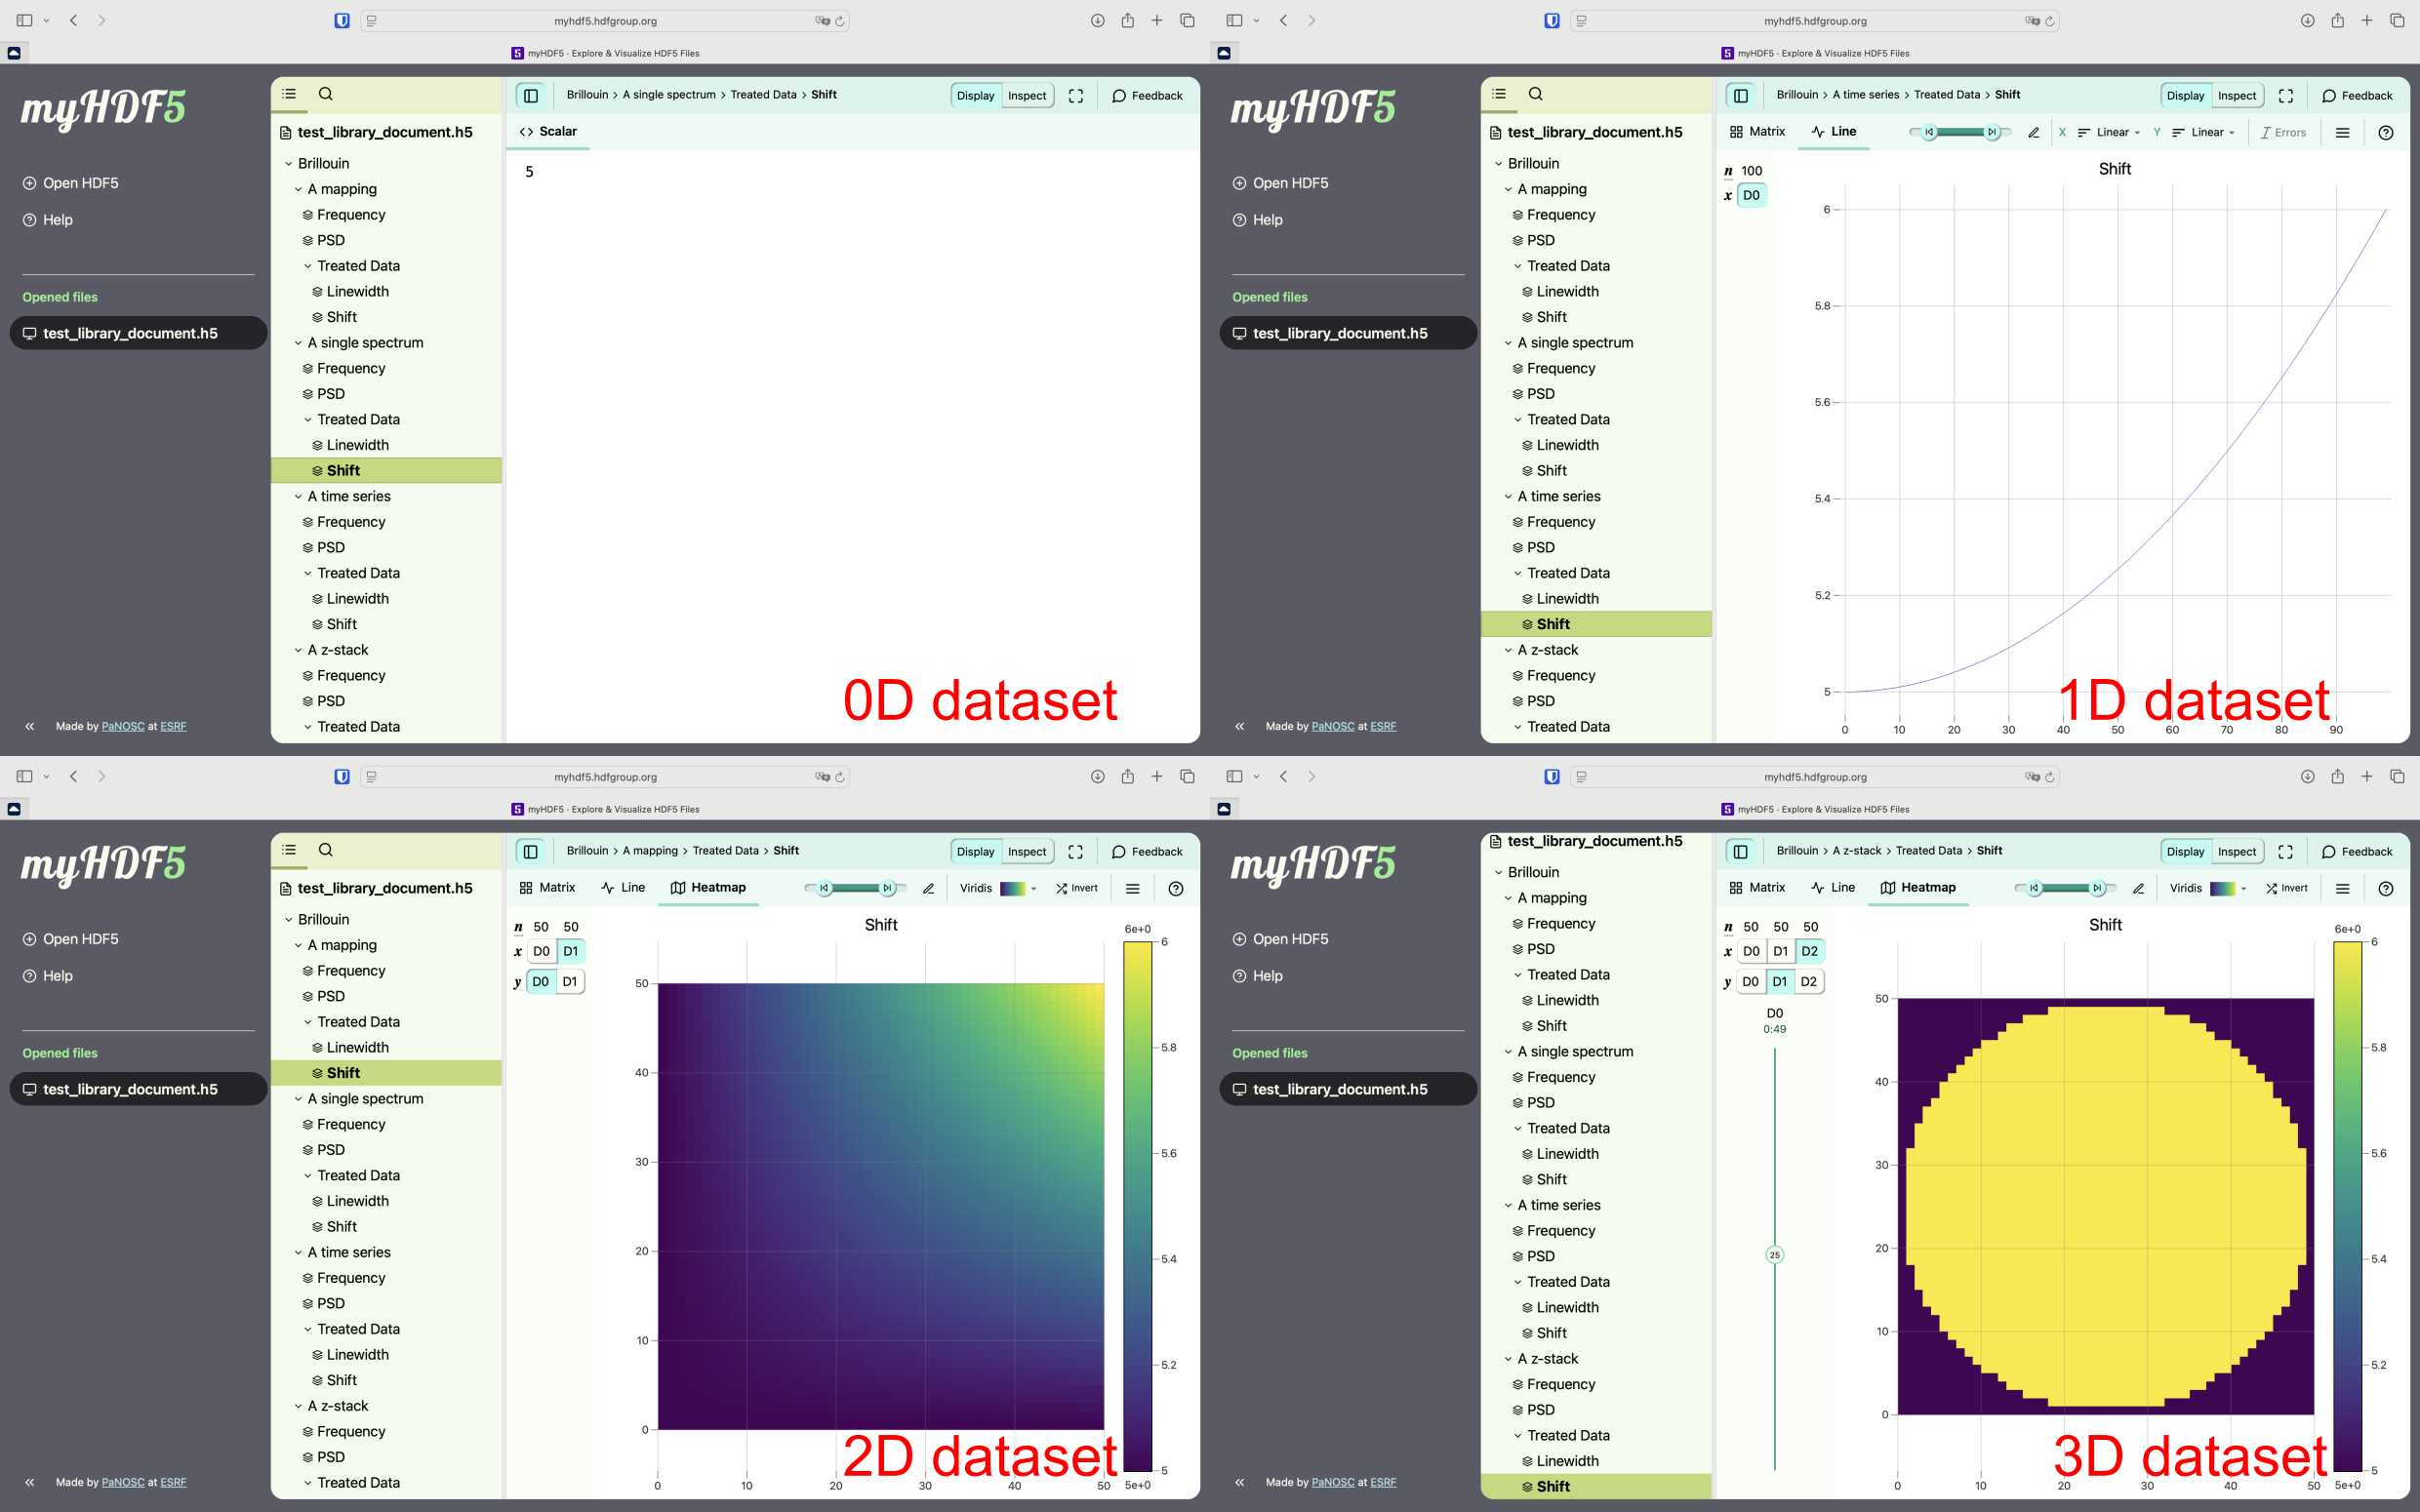
\includegraphics[width=\textwidth]{img/MyHDF5_visualizer.png}
    \caption{Visualizing the datasets using the MyHDF5 web application} 
    \label{fig:my_hdf5_datasets}
\end{figure}

\subsection{Using Panoply}

Panoply is an application developed by NASA to visualize geo-referenced data and more generally HDF5 files. It can be downloaded for free at this link: \url{https://www.giss.nasa.gov/tools/panoply/}. 

Here are some screenshots of the application with the example file we created in this tutorial: 

\begin{figure}[H]
    \centering
    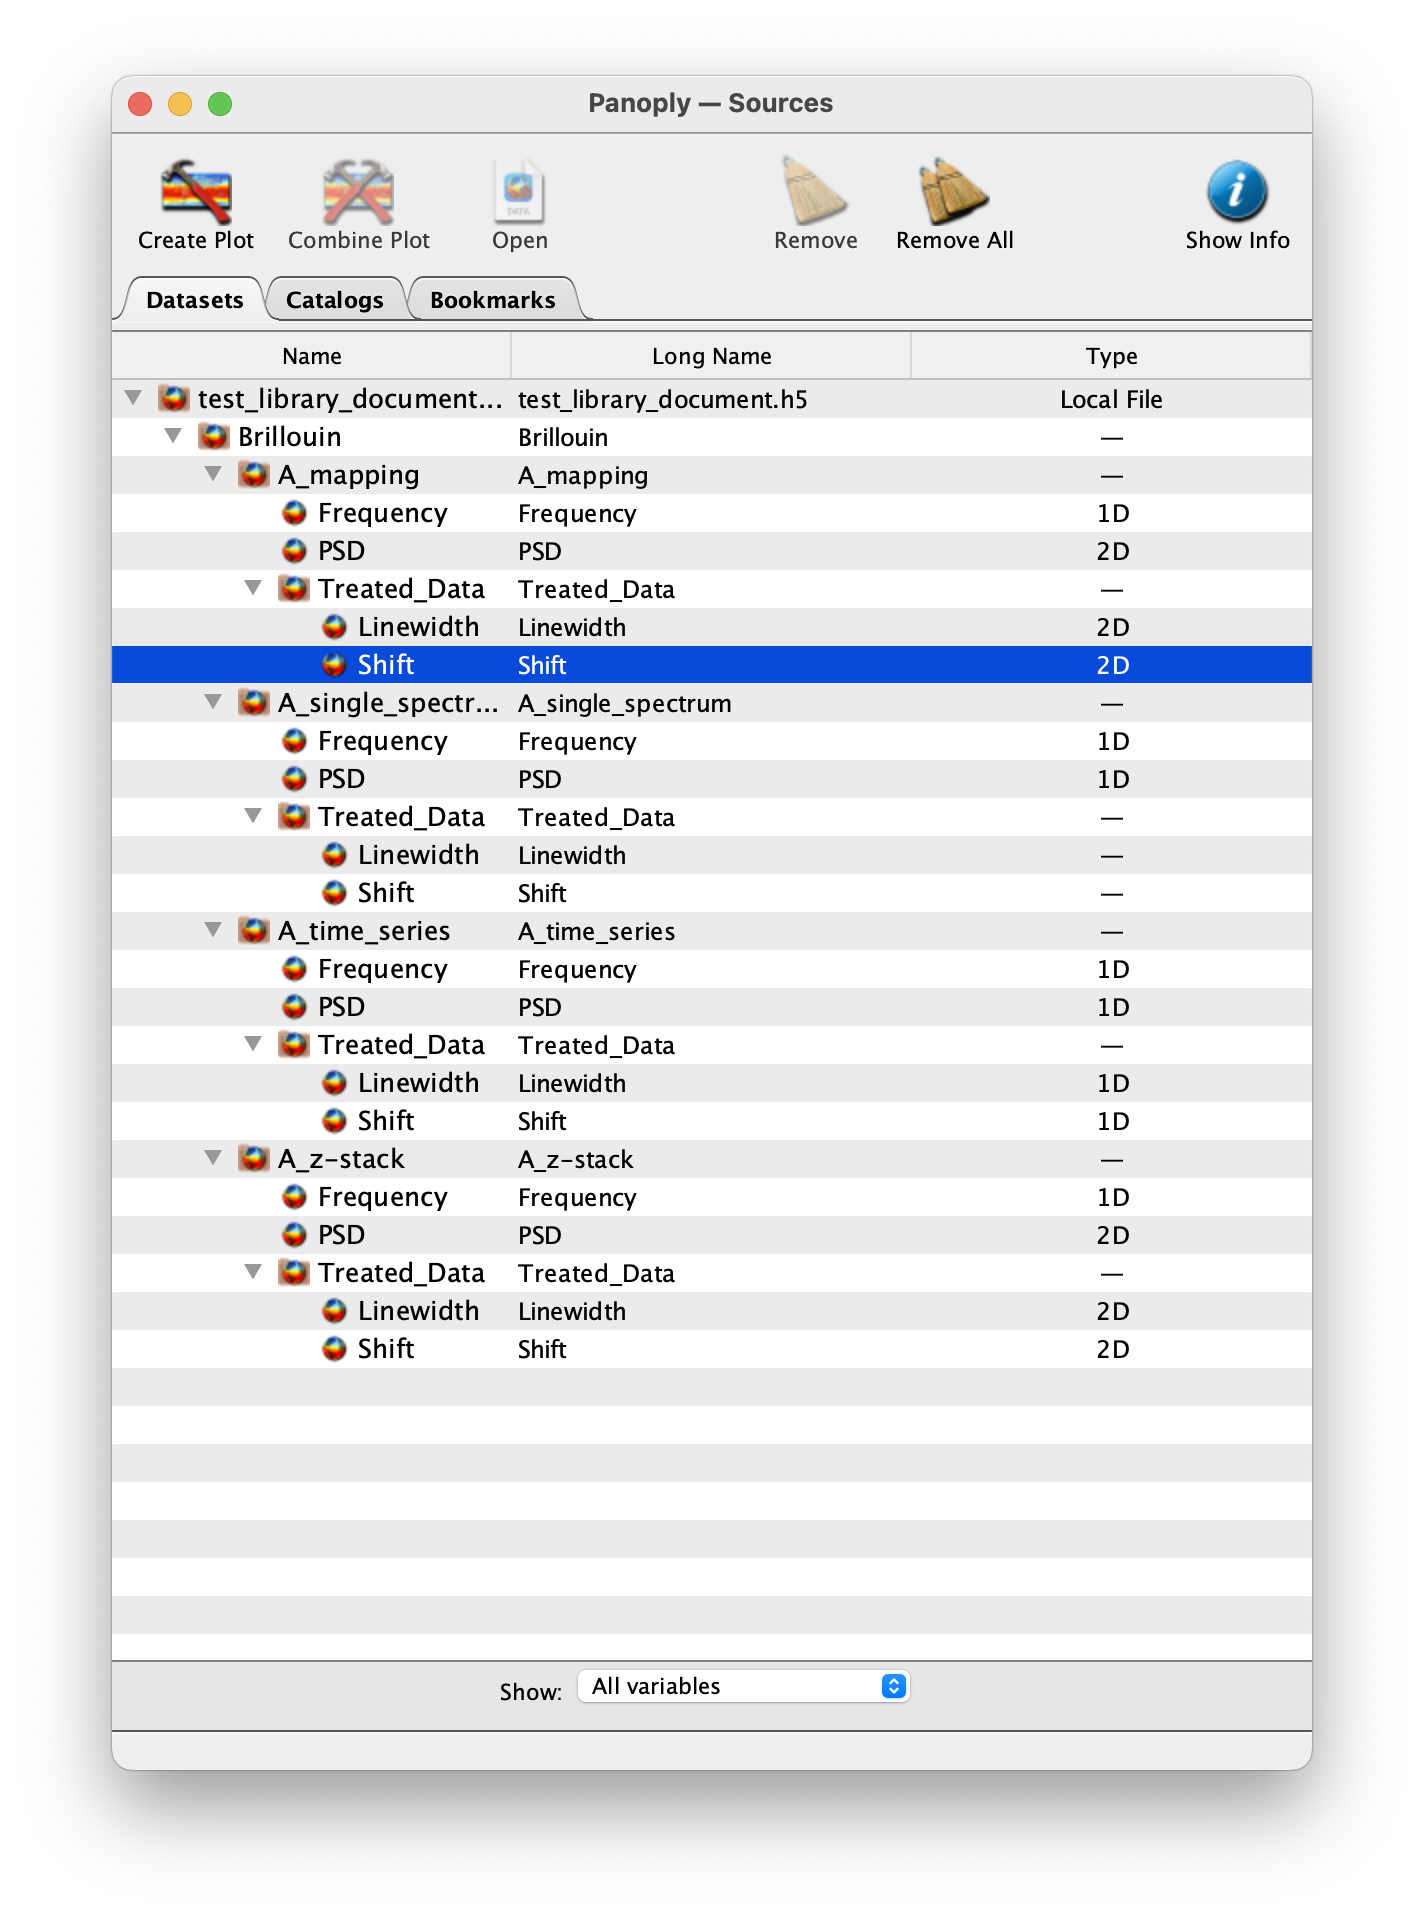
\includegraphics[width=0.4\textwidth]{img/Panoply_developed_structure.png}
    \caption{A simple visualization of the HDF5 file structure using the Panoply application} 
    \label{fig:panoply_developed_structure}
\end{figure}

\begin{figure}[H]
    \centering
    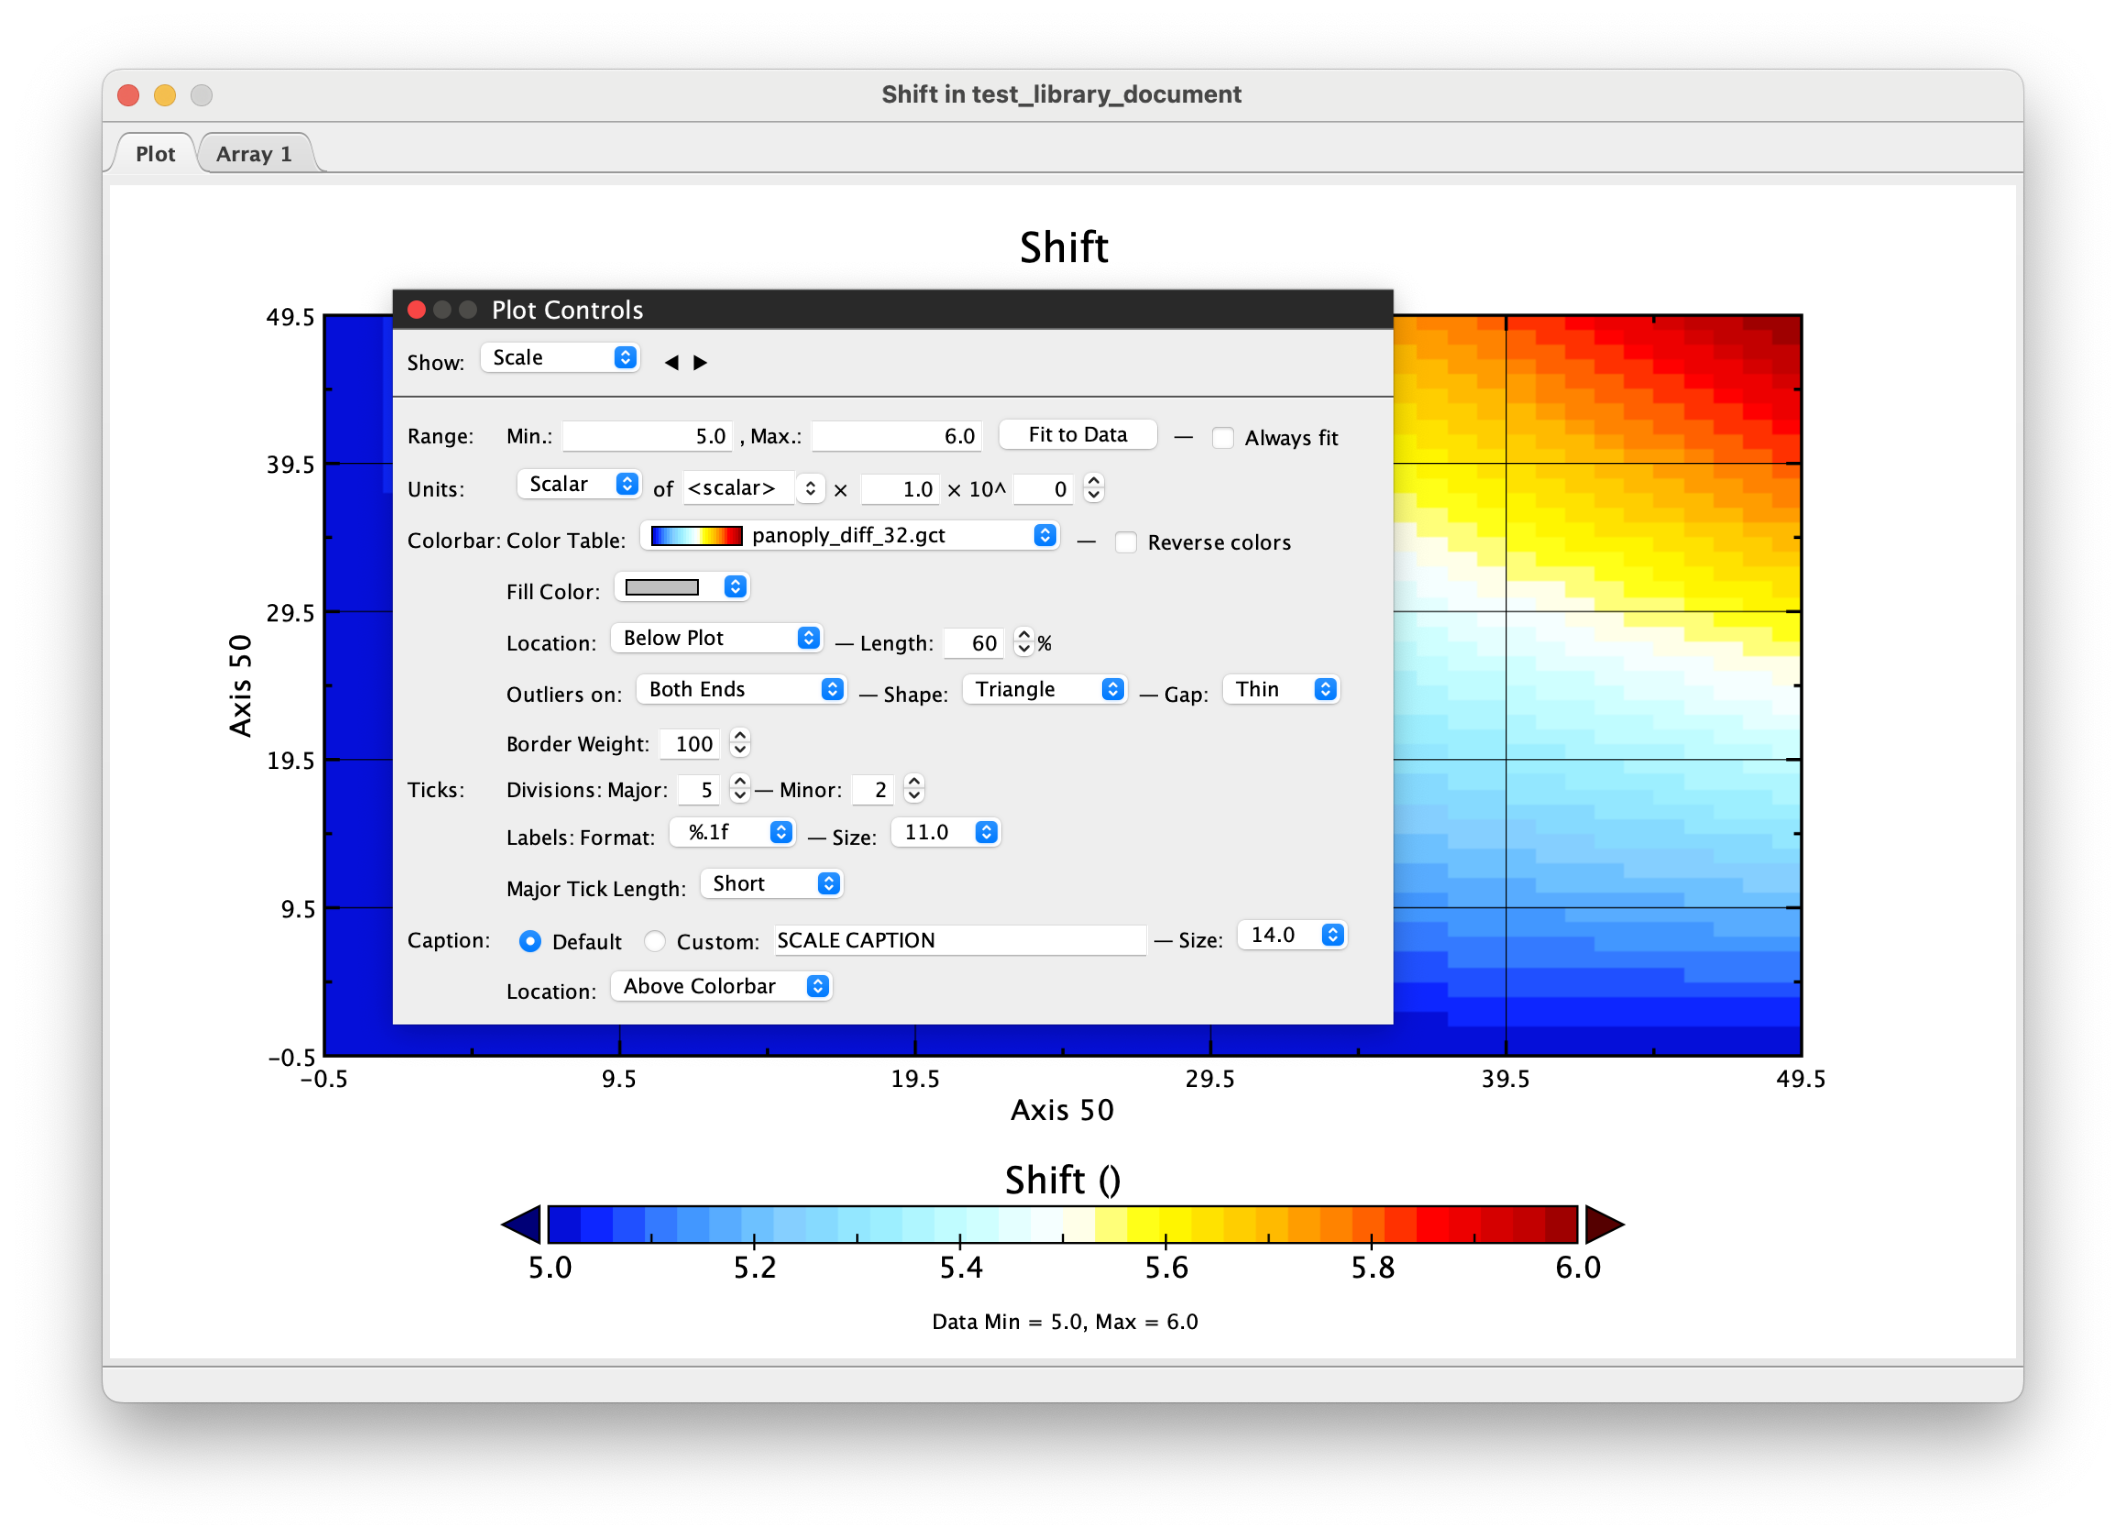
\includegraphics[width=0.7\textwidth]{img/Panoply_viewer.png}
    \caption{Visualizing datasets using the Panoply application} 
    \label{fig:panoply_viewer}
\end{figure}

\section{The HDF5\_BLS\_GUI}

The HDF5\_BLS\_GUI is a graphical user interface for the HDF5\_BLS package, designed to facilitate the exploration and analysis of HDF5 files. It provides a user-friendly environment for users to create and interact with their data. The GUI is meant to evolve to allow users to treat their data from it, but these developments are still in a beta phase. 

To use the GUI, you need to install the package. Follow the instructions below:

\begin{itemize}
    \item Clone the repository: \texttt{git clone https://github.com/yourusername/HDF5\_BLS.git}
    \item Navigate to the directory: \texttt{cd HDF5\_BLS}
    \item Install the packages for the library: \texttt{pip install -r requirements\_library.txt}
    \item Install the packages for the GUI: \texttt{pip install -r requirements\_GUI.txt}
    \item Run the GUI: \texttt{python HDF5\_BLS\_GUI/main.py}
\end{itemize}

You should see the HDF5\_BLS\_GUI window appear on your screen (figure \ref{fig:gui_main_window}).

\begin{figure}[H]
    \centering
    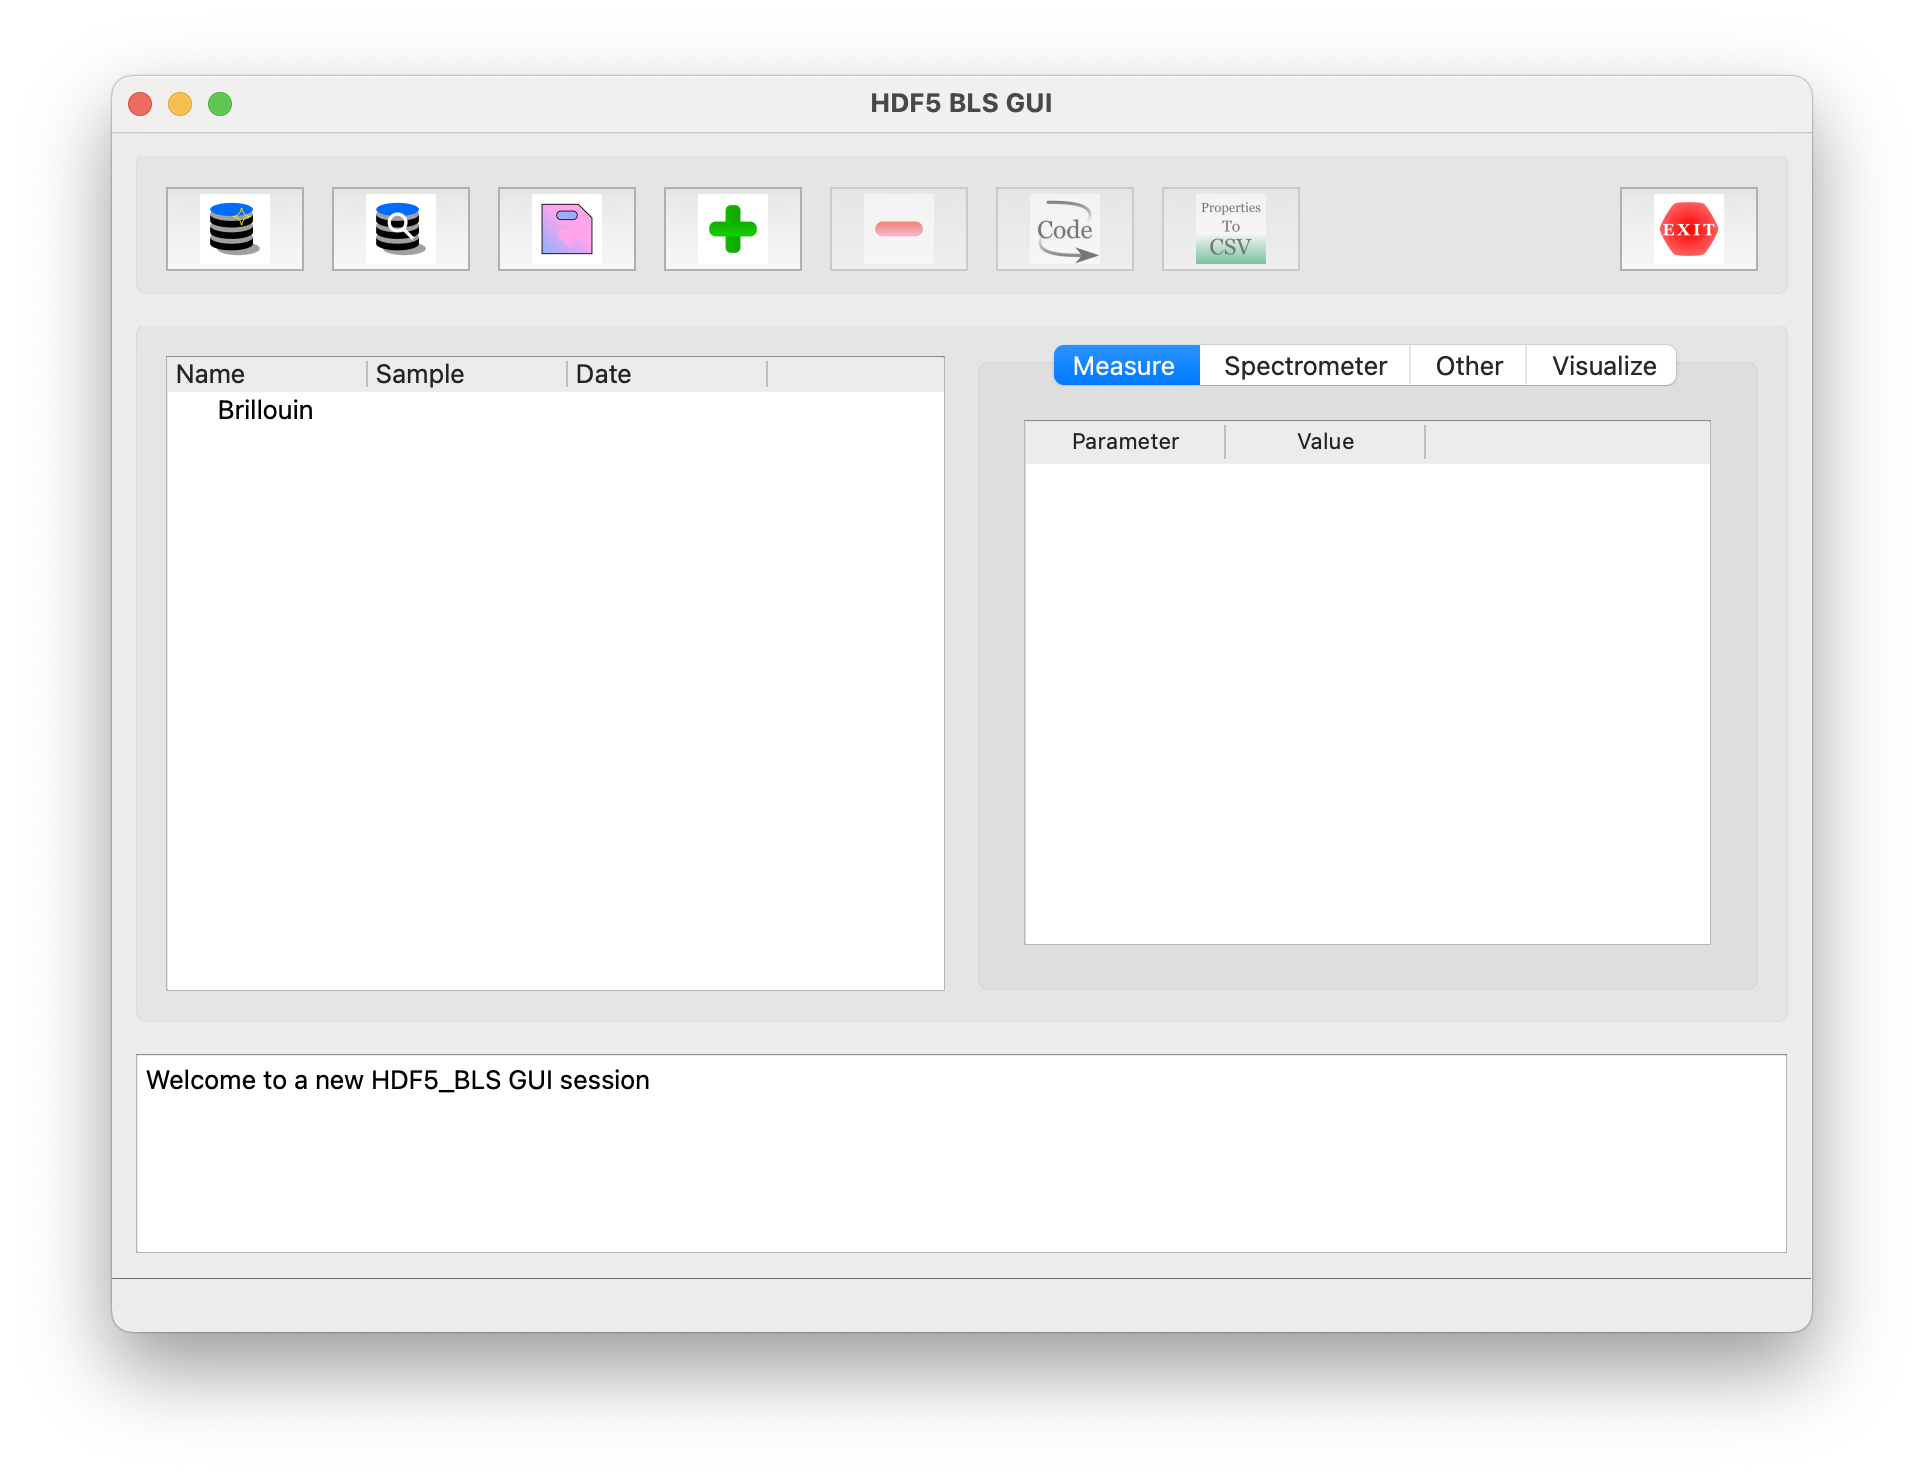
\includegraphics[width=0.8\textwidth]{img/HDF5_BLS_GUI_welcome.png}
    \caption{The welcome window of the HDF5\_BLS\_GUI}
    \label{fig:gui_main_window}
\end{figure}

You can then drag and drop your data into the left panel if its addition is already supported by the GUI. If not, you'll be forced to add it from script. 

You can then structure your file by creating groups, renaming them, dragging files from groups to groups, and generally use the GUI as you would a normal file explorer.

When adding a data, the GUI automatically creates a new group in the HDF5 file. You can change the name of the group by double clicking on it. You can also drag excel files with properties to the right panel to apply metadata to groups.

You can of course drag and drop the BrimX file we have created in this tutorial to the left panel to see its structure (figure \ref{fig:brimx_structure}).

\begin{figure}[H]
    \centering
    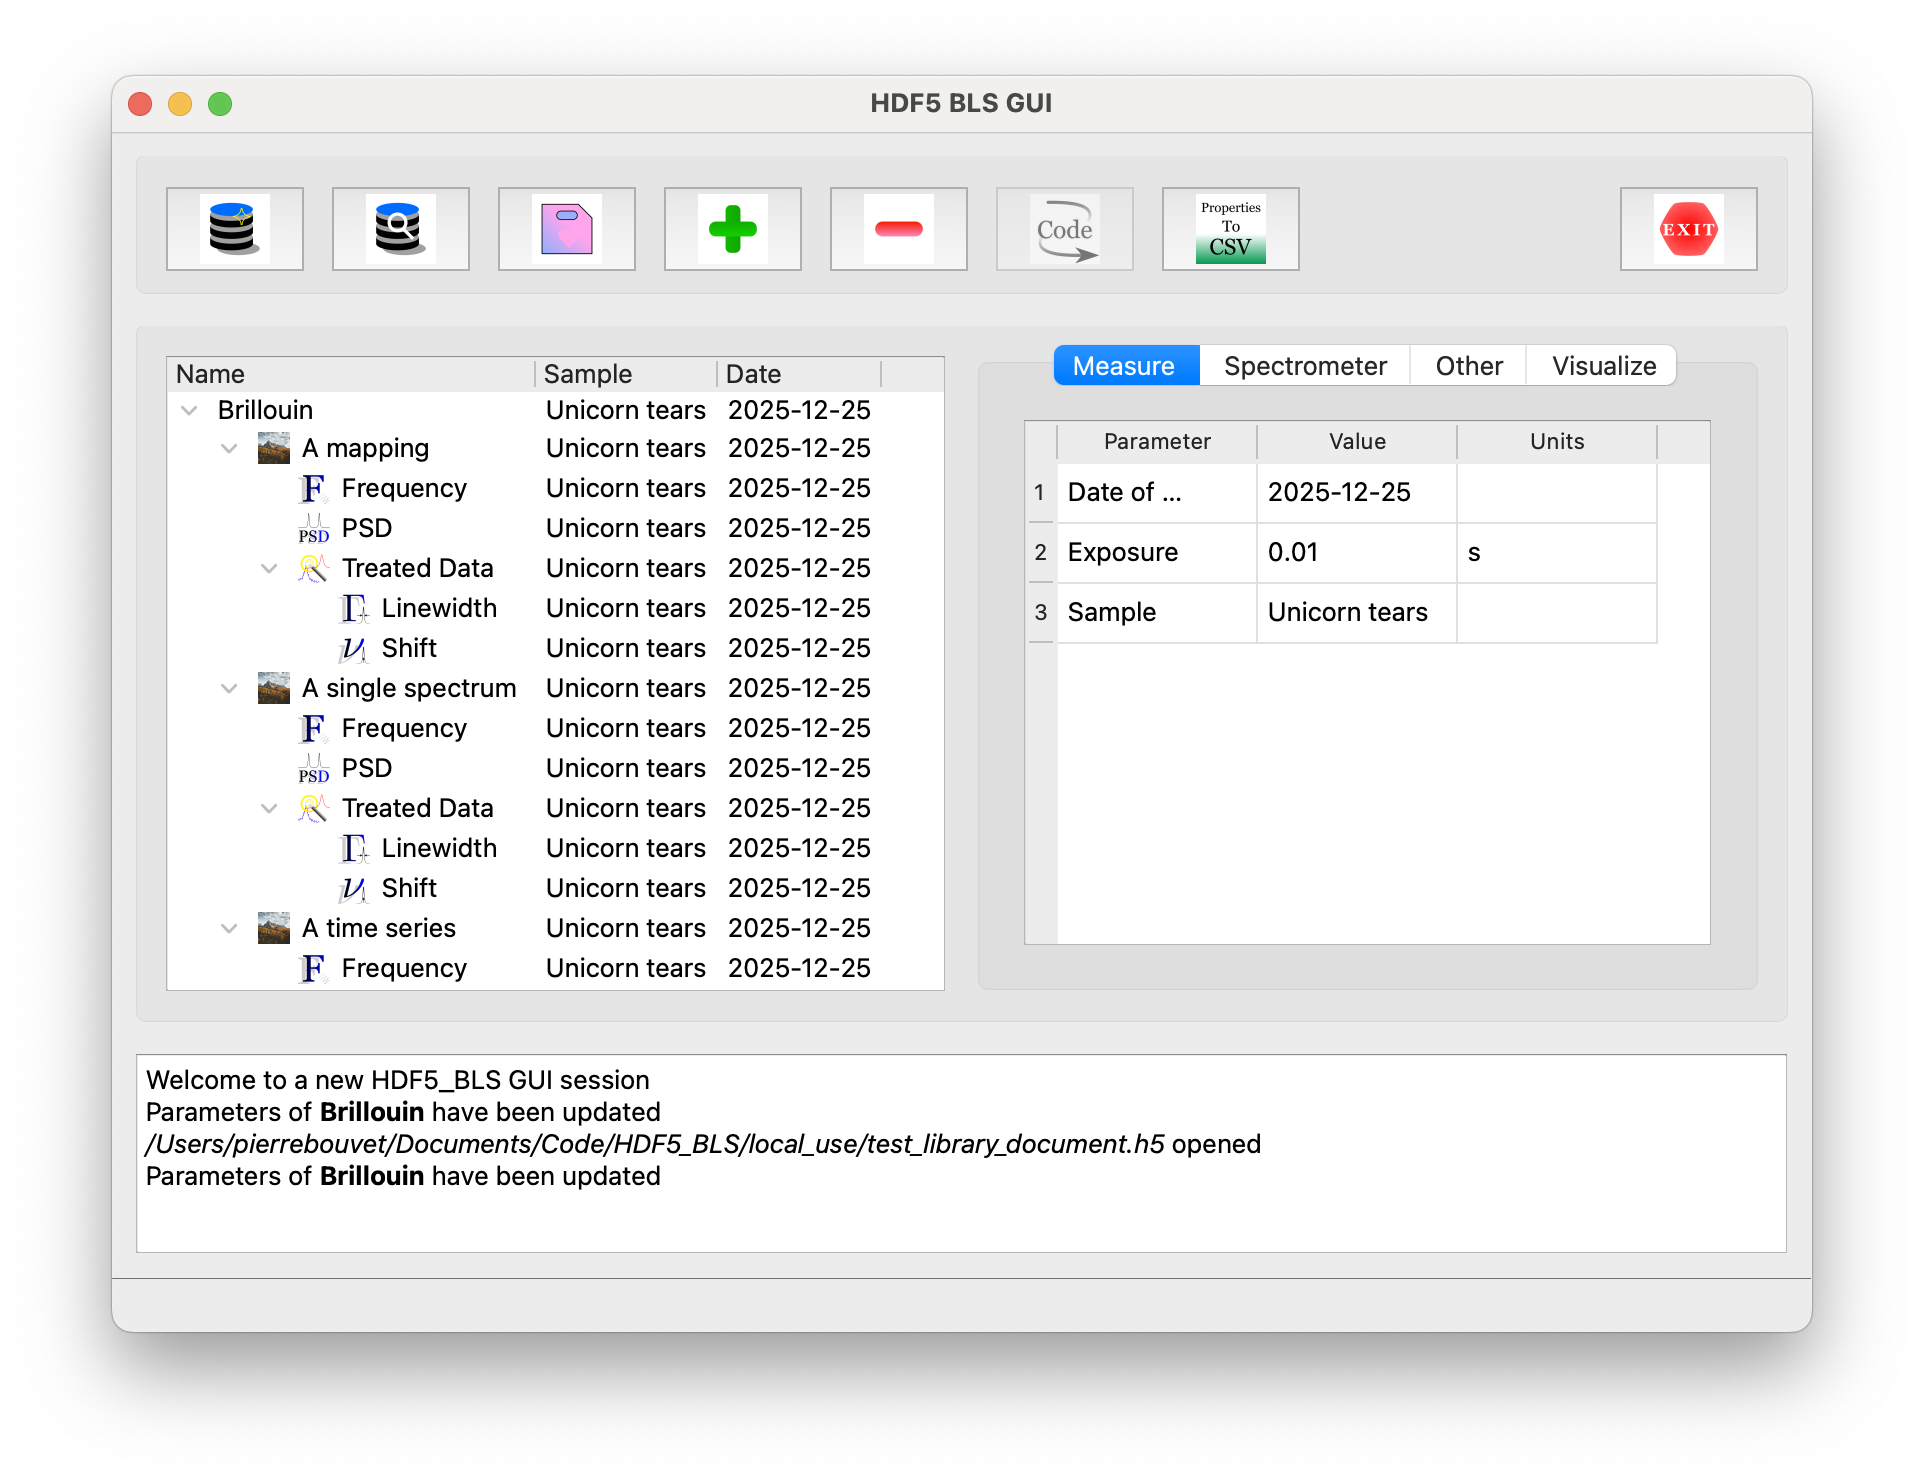
\includegraphics[width=0.8\textwidth]{img/HDF5_BLS_GUI_BrimX_structure.png}
    \caption{The structure of the example BrimX file in the HDF5\_BLS\_GUI}
    \label{fig:brimx_structure}
\end{figure}

This GUI is still in development, so don't hesitate to report bugs or suggest features on the GitHub repository: \url{https://github.com/bio-brillouin/HDF5_BLS/issues}.

\section{Ending remarks}

In this tutorial, we have covered the basics of using the HDF5\_BLS\_GUI for exploring and managing HDF5 files. We encourage you to experiment with the GUI and provide feedback to help us improve it. You can directly contact me at \href{mailto:pierre.bouvet@meduniwien.ac.at}{pierre.bouvet@meduniwien.ac.at} !

\vspace{5\baselineskip}

\begin{center}
\textbf{Thank you for your help! Happy Brillouin data handling!}
\end{center}

\end{document}